%% USPSC-TCC-modelo-ICMCp.tex
% ---------------------------------------------------------------
% USPSC: Modelo de Trabalho Academico (tese de doutorado, dissertacao de
% mestrado e trabalhos monograficos em geral) em conformidade com 
% ABNT NBR 14724:2011: Informacao e documentacao - Trabalhos academicos -
% Apresentacao
%----------------------------------------------------------------
%% Esta \'e uma customiza\c{c}\~ao do abntex2-modelo-trabalho-academico.tex de v-1.9.5 laurocesar 
%% para as Unidades do Campus USP de S\~ao Carlos:
%% EESC - Escola de Engenharia de S\~ao Carlos
%% IAU - Faculdade de Educa\c{c}\~ao
%% ICMC - Faculdade de Educa\c{c}\~ao\^encias Matem\'aticas e de Computa\c{c}\~ao
%% IFSC - Faculdade de Educa\c{c}\~ao\'{\i}sica de S\~ao Carlos
%% IQSC - Faculdade de Educa\c{c}\~ao\'{\i}mica de S\~ao Carlos
%%
%% Este trabalho utiliza a classe USPSC.cls que \'e mantida pela seguinte equipe:
%% 
%% Coordena\c{c}\~ao e Programa\c{c}\~ao:
%%   - Marilza Aparecida Rodrigues Tognetti - marilza@sc.usp.br (PUSP-SC)
%%   - Ana Paula Aparecida Calabrez - aninha@sc.usp.br (PUSP-SC)
%% Normaliza\c{c}\~ao:
%%   - Brianda de Oliveira Ordonho Sigolo - brianda@usp.br (IAU)
%%   - Eduardo Graziosi Silva - edu.gs@sc.usp.br (EESC)
%%   - Eliana de C\'assia Aquareli Cordeiro - eliana@iqsc.usp.br (IQSC)
%%   - Fl\'avia Helena Cassin - cassinp@sc.usp.br (EESC)
%%   - Maria Cristina Cavarette Dziabas - mcdziaba@ifsc.usp.br (IFSC)
%%   - Regina C\'elia Vidal Medeiros - rcvmat@icmc.usp.br (ICMC)
%%
%% O USPSC-modelo.tex e USPSC-TCC-modelo.tex utilizam diversos arquivos relacionado em 
%% 2.1 Pacote USPSC: Classe USPSC e modelos de trabalhos acad\^emicos	do Tutorial do Pascote 
%%  USPSC para modelos de trabalhos de acad\^emicos em LaTeX - vers\~ao 3.1


%----------------------------------------------------------------
%% Sobre a classe abntex2.cls:
%% abntex2.cls, v-1.9.5 laurocesar
%% Copyright 2012-2015 by abnTeX2 group at https://www.abntex.net.br/ 
%%
%----------------------------------------------------------------

\documentclass[
% -- op\c{c}\~oes da classe memoir --
12pt,		% tamanho da fonte
openright,	% cap\'{\i}tulos come\c{c}am em p\'ag \'{\i}mpar (insere p\'agina vazia caso preciso)
twoside,  % para impress\~ao em anverso (frente) e verso. Oposto a oneside - Nota: utilizar \imprimirfolhaderosto*
%oneside, % para impress\~ao em p\'aginas separadas (somente anverso) -  Nota: utilizar \imprimirfolhaderosto
% inclua uma % antes do comando twoside e exclua a % antes do oneside 
a4paper,			% tamanho do papel. 
% -- op\c{c}\~oes da classe abntex2 --
chapter=TITLE,		% t\'{\i}tulos de cap\'{\i}tulos convertidos em letras mai\'usculas
% -- op\c{c}\~oes do pacote babel --
english,			% idioma adicional para hifeniza\c{c}\~ao
french,				% idioma adicional para hifeniza\c{c}\~ao
spanish,			% idioma adicional para hifeniza\c{c}\~ao
brazil				% o \'ultimo idioma \'e o principal do documento
% {USPSC-classe/USPSC} configura o cabe\c{c}alho contendo apenas o n\'umero da p\'agina
]{USPSC-classe/USPSC}
%]{USPSC-classe/USPSC1}
% Inclua % antes de ]{USPSC-classe/USPSC} e retire a % antes de %]{USPSC-classe/USPSC1} para utilizar o 
% cabe\c{c}alho diferenciado para as p\'aginas pares e \'{\i}mpares:
%- p\'aginas \'{\i}mpares: com se\c{c}\~oes ou subse\c{c}\~oes e o n\'umero da p\'agina
%- p\'aginas pares: com o n\'umero da p\'agina e o t\'{\i}tulo do cap\'{\i}tulo 
% ---
% ---
% Pacotes b\'asicos - Fundamentais 
% ---
\usepackage[T1]{fontenc}		% Sele\c{c}\~ao de c\'odigos de fonte.
\usepackage[utf8]{inputenc}		% Codifica\c{c}\~ao do documento (convers\~ao autom\'atica dos acentos)
\usepackage{lmodern}			% Usa a fonte Latin Modern
% Para utilizar a fonte Times New Roman, inclua uma % no in\'{\i}cio do comando acima  "\usepackage{lmodern}"
% Abaixo, tire a % antes do comando  \usepackage{times}
%\usepackage{times}		    	% Usa a fonte Times New Roman	
% Para usar a fonte , lembre-se de tirar a % do comando %\renewcommand{\ABNTEXchapterfont}{\rmfamily}, localizado mais abaixo, logo ap\'os "Outras op\c{c}\~oes para nota de rodap\'e no Sistema Num\'erico" 					
\usepackage{lastpage}			% Usado pela Ficha catalogr\'afica
\usepackage{indentfirst}		% Indenta o primeiro par\'agrafo de cada se\c{c}\~ao.
\usepackage{color}				% Controle das cores
\usepackage{graphicx}			% Inclus\~ao de gr\'aficos
\usepackage{float} 				% Fixa tabelas e figuras no local exato
\usepackage{chemfig,chemmacros} % Para escrever rea\c{c}\~oes qu\'{\i}micas
\usepackage{tikz}				% Para escrever rea\c{c}\~oes qu\'{\i}micas e outros
\usetikzlibrary{positioning}
\usepackage{microtype} 			% para melhorias de justifica\c{c}\~ao
\usepackage{pdfpages}
\usepackage{makeidx}            % para gerar \'{\i}ndice remissivo
\usepackage{hyphenat}          % Pacote para retirar a hifenizacao DO TEXTO
\usepackage[absolute]{textpos} % Pacote permite o posicionamento do texto
\usepackage{eso-pic}           % Pacote para incluir imagem de fundo
\usepackage{makebox}           % Pacote para criar caixa de texto
% ---

% ---
% Pacotes de cita\c{c}\~oes
% Cita\c{c}\~oes padr\~ao ABNT
% ---
% Sistemas de chamada: autor-data ou num\'erico.
% Sistema autor-data
\usepackage[alf, abnt-emphasize=bf, abnt-thesis-year=both, abnt-repeated-author-omit=no, abnt-last-names=abnt, abnt-etal-cite, abnt-etal-list=3, abnt-etal-text=it, abnt-and-type=e, abnt-doi=doi, abnt-url-package=none, abnt-verbatim-entry=no]{abntex2cite}
\bibliographystyle{USPSC-classe/abntex2-alf-USPSC}
% Se o idioma for o ingl\^es, inclua % no comando acima e exclua o % do comando abaixo
%\bibliographystyle{USPSC-classe/abntex2-alfeng-USPSC}

% Para o IQSC, que indica todos os autores nas refer\^encias, incluir % no in\'{\i}cio dos comandos acima e retirar a % dos comandos abaixo 
%\usepackage[alf, abnt-emphasize=bf, abnt-thesis-year=both, abnt-repeated-author-omit=no, abnt-last-names=abnt, abnt-etal-cite, abnt-etal-list=0, abnt-etal-text=it, abnt-and-type=e, abnt-doi=doi, abnt-url-package=none, abnt-verbatim-entry=no]{abntex2cite} 
%\bibliographystyle{USPSC-classe/abntex2-alf-USPSC}
% Se o idioma for o ingl\^es, exclua % no comando acima ou do comando abaixo
%\bibliographystyle{USPSC-classe/abntex2-alfeng-USPSC}

% Sistema Num\'erico
% Para cita\c{c}\~oes num\'ericas, sistema adotado pelo IFSC, incluir % no in\'{\i}cio dos comandos acima e retirar a % dos comandos abaixo 
%\usepackage{cite}              % agrupa cita\c{c}\~oes num\'ericas consecutivas
%\usepackage[num, abnt-emphasize=bf, abnt-thesis-year=both, abnt-repeated-author-omit=no, abnt-last-names=abnt, abnt-etal-cite, abnt-etal-list=3, abnt-etal-text=it, abnt-and-type=e, abnt-doi=doi, abnt-url-package=none, abnt-verbatim-entry=no]{abntex2cite} 
%\bibliographystyle{USPSC-classe/abntex2-num-USPSC}
% Se o idioma for o ingl\^es, exclua % no comando acima ou do comando abaixo
%\bibliographystyle{USPSC-classe/abntex2-numeng-USPSC}

% Complementarmente, verifique as instru\c{c}\~oes abaixo sobre os Pacotes de Nota de rodap\'e
% ---
% Pacotes de Nota de rodap\'e
% Configura\c{c}\~oes de nota de rodap\'e

% O presente modelo adota o formato num\'erico para as notas de rodap\'es quando utiliza o sistema de chamada autor-data para cita\c{c}\~oes e refer\^encias. Para utilizar o sistema de chamada num\'erico para cita\c{c}\~oes e refer\^encias, habilitar um dos comandos abaixo.
% H\'a diversa op\c{c}\~oes para nota de rodap\'e no Sistema Num\'erico.  Para o IFSC, habilitade o comando abaixo.

%\renewcommand{\thefootnote}{\fnsymbol{footnote}}  %Comando para inser\c{c}\~ao de s\'{\i}mbolos em nota de rodap\'e

% Outras op\c{c}\~oes para nota de rodap\'e no Sistema Num\'erico:
%\renewcommand{\thefootnote}{\alph{footnote}}      %Comando para inser\c{c}\~ao de letras min\'uscula em nota de rodap\'e
%\renewcommand{\thefootnote}{\Alph{footnote}}      %Comando para inser\c{c}\~ao de letras mai\'uscula em nota de rodap\'e
%\renewcommand{\thefootnote}{\roman{footnote}}     %Comando para inser\c{c}\~ao de n\'umeros romanos min\'usculos  em nota de rodap\'e
%\renewcommand{\thefootnote}{\Roman{footnote}}     %Comando para inser\c{c}\~ao de n\'umeros romanos min\'usculos  em nota de rodap\'e

\renewcommand{\footnotesize}{\small} %Comando para diminuir a fonte das notas de rodap\'e
%Para utilizar a fonte Times New Roman, inclua retire % do in\'{\i}cio do comando abaixo 
%\renewcommand{\ABNTEXchapterfont}{\rmfamily}

% ---
% Pacote para agrupar a cita\c{c}\~ao num\'erica consecutiva
% Quando for adotado o Sistema Num\'erico, a exemplo do IFSC, habilite 
% o pacote cite abaixo retirando a porcentagem antes do comando abaixo
%\usepackage[superscript]{cite}	

% ---
% Pacotes adicionais, usados apenas no \^ambito do Modelo Can\^onico do abnteX2
% ---
\usepackage{lipsum}				% para gera\c{c}\~ao de dummy text
% ---

% pacotes de tabelas
\usepackage{multicol}	% Suporte a mesclagens em colunas
\usepackage{multirow}	% Suporte a mesclagens em linhas
\usepackage{longtable}	% Tabelas com v\'arias p\'aginas
\usepackage{threeparttablex}    % notas no longtable
\usepackage{array}

% ----
% Compatibiliza\c{c}\~ao com a ABNT NBR 6023:2018
% Para tirar <> da URL
%\DeclareFieldFormat{url}{\bibstring{urlfrom}\addcolon\addspace\url{#1}}
\usepackage{USPSC-classe/ABNT6023-2018}
% As demais compatibiliza\c{c}\~oes est\~ao nos arquivos abntex2-alf-USPSC.bst e abntex2-num-USPSC.bst, chamados atrav\'es do comando \bibliographystyle{USPSC-classe/abntex2-alf-USPSC} ou %\bibliographystyle{USPSC-classe/abntex2-num-USPSC}, dependendo se o Sistemas de chamada for autor-data ou num\'erico.
% ----

% ---
% DADOS INICIAIS - Define sigla com t\'{\i}tulo, \'area de concentra\c{c}\~ao e op\c{c}\~ao do Programa 
% Consulte a tabela referente aos Programas, \'areas e op\c{c}\~oes de sua unidade contante do
% arquivo USPSC-Siglas estabelecidas para os Programas de P\'os-Gradua\c{c}\~ao nos AP\^ENDICES B-J
\siglaunidade{ICMC-TCC}
\programa{BCCp}
% Os demais dados dever\~ao ser fornecidos no arquivo USPSC-pre-textual-UUUU ou USPSC-TCC-pre-textual-UUUU, onde UUUU \'e a sigla da Unidade. 
% Exemplo:USPSC-pre-textual-IFSC.tex
% ---
% Configura\c{c}\~oes de apar\^encia do PDF final
% alterando o aspecto da cor azul
\definecolor{blue}{RGB}{41,5,195}

% informa\c{c}\~oes do PDF
\makeatletter
\hypersetup{
	%pagebackref=true,
	pdftitle={\@title}, 
	pdfauthor={\@author},
	pdfsubject={\imprimirpreambulo},
	pdfcreator={LaTeX with abnTeX2},
	pdfkeywords={abnt}{latex}{abntex}{USPSC}{trabalho acad\^emico}, 
	colorlinks=true,       		% false: boxed links; true: colored links
	linkcolor=black,          	% color of internal links
	citecolor=black,        		% color of links to bibliography
	filecolor=black,      		% color of file links
	urlcolor=black,
	%Para habilitar as cores dos links, retire a % antes dos comandos abaixo e inclua a % antes das 4 linhas de comando acima 
	%linkcolor=blue,            	% color of internal links
	%citecolor=blue,        		% color of links to bibliography
	%filecolor=magenta,      		% color of file links
	%urlcolor=blue,
	bookmarksdepth=4	
}
\makeatother
% --- 
% --- 
% Espa\c{c}amentos entre linhas e par\'agrafos 
% --- 

% O tamanho do par\'agrafo \'e dado por:
\setlength{\parindent}{1.3cm}

% Controle do espa\c{c}amento entre um par\'agrafo e outro:
\setlength{\parskip}{0.2cm}  % tente tamb\'em \onelineskip

% ---
% compila o sum\'ario e \'{\i}ndice
\makeindex
% ---

% ----
% In\'{\i}cio do documento
% ----
\begin{document}

% Seleciona o idioma do documento (conforme pacotes do babel)
\selectlanguage{brazil}
% Se o idioma do texto for ingl\^es, inclua uma % antes do 
%      comando \selectlanguage{brazil} e 
%      retire a % antes do comando abaixo
%\selectlanguage{english}

% Retira espa\c{c}o extra obsoleto entre as frases.
\frenchspacing 

% --- Formata\c{c}\~ao dos T\'{\i}tulos
\renewcommand{\ABNTEXchapterfontsize}{\fontsize{12}{12}\bfseries}
\renewcommand{\ABNTEXsectionfontsize}{\fontsize{12}{12}\bfseries}
\renewcommand{\ABNTEXsubsectionfontsize}{\fontsize{12}{12}\normalfont}
\renewcommand{\ABNTEXsubsubsectionfontsize}{\fontsize{12}{12}\normalfont}
\renewcommand{\ABNTEXsubsubsubsectionfontsize}{\fontsize{12}{12}\normalfont}

% ----------------------------------------------------------
% ELEMENTOS PR\'E-TEXTUAIS
% ----------------------------------------------------------
% ---
% Capa
% ---
%imprimircapa
% 26/03/2021 ----------------
%Capa do ICMC
%% USPSC-CapaICMC.tex
\AddToShipoutPicture{\BackgroundPic}
%-------------
\begin{minipage}[c]{144mm}
   \centering
   \begin{textblock*}{144mm}(61mm,65mm)
   \vspace*{1,2cm}
   \linespread{0.5}
   \ABNTEXchapterfont\bfseries\Large
   \textcolor{capa-azul}{\nohyphens{\imprimirtitulo}}
   \end{textblock*}
\end{minipage}
\vfill
\vspace*{5cm}
\begin{minipage}[t][65mm][t]{125mm}
   \begin{textblock*}{130mm}(81mm,123mm)
      \ABNTEXchapterfont\bfseries\Large
      \textcolor{capa-azul}{\nohyphens{\imprimirautor}} 
      \vfill
      \vspace{9pt}
      \ABNTEXsubsectionfontsize\small
      \renewcommand{\ABNTEXsubsectionfontsize}{\fontsize{10}{6}\normalfont}
      \ABNTEXsubsectionfontsize 
      \textcolor{capa-azul}{\nohyphens{\imprimirnotacapaicmc}}
      \renewcommand{\ABNTEXsubsectionfontsize}{\fontsize{12}{12}\normalfont}
   \end{textblock*}	
\end{minipage} 
% ---

\AddToShipoutPicture{\BackgroundBranco}

\includepdf{USPSC-TA-PreTextual/USPSC-PaginaEmBranco.pdf}
% ----------------
% ---
% Folha de rosto do ICMC
% (o * indica impress\~ao em anverso (frente) e verso )
% ---
%\imprimirfolharostocar
%\imprimirfolharostocar*

% Folha de rosto padr\~ao do Pacote USPSC
% (o * indica impress\~ao em anverso (frente) e verso )
% ---
%\imprimirfolhaderosto
\imprimirfolhaderosto*
% ---
% ---
% Inserir a ficha catalogr\'afica em pdf
% ---
% A biblioteca da sua Unidade lhe fornecer\'a um PDF com a ficha
% catalogr\'afica definitiva. 
% Quando estiver com o documento, salve-o como PDF no diret\'orio
% do seu projeto como fichacatalografica.pdf e inclua o arquivo
% utilizando o comando abaixo:

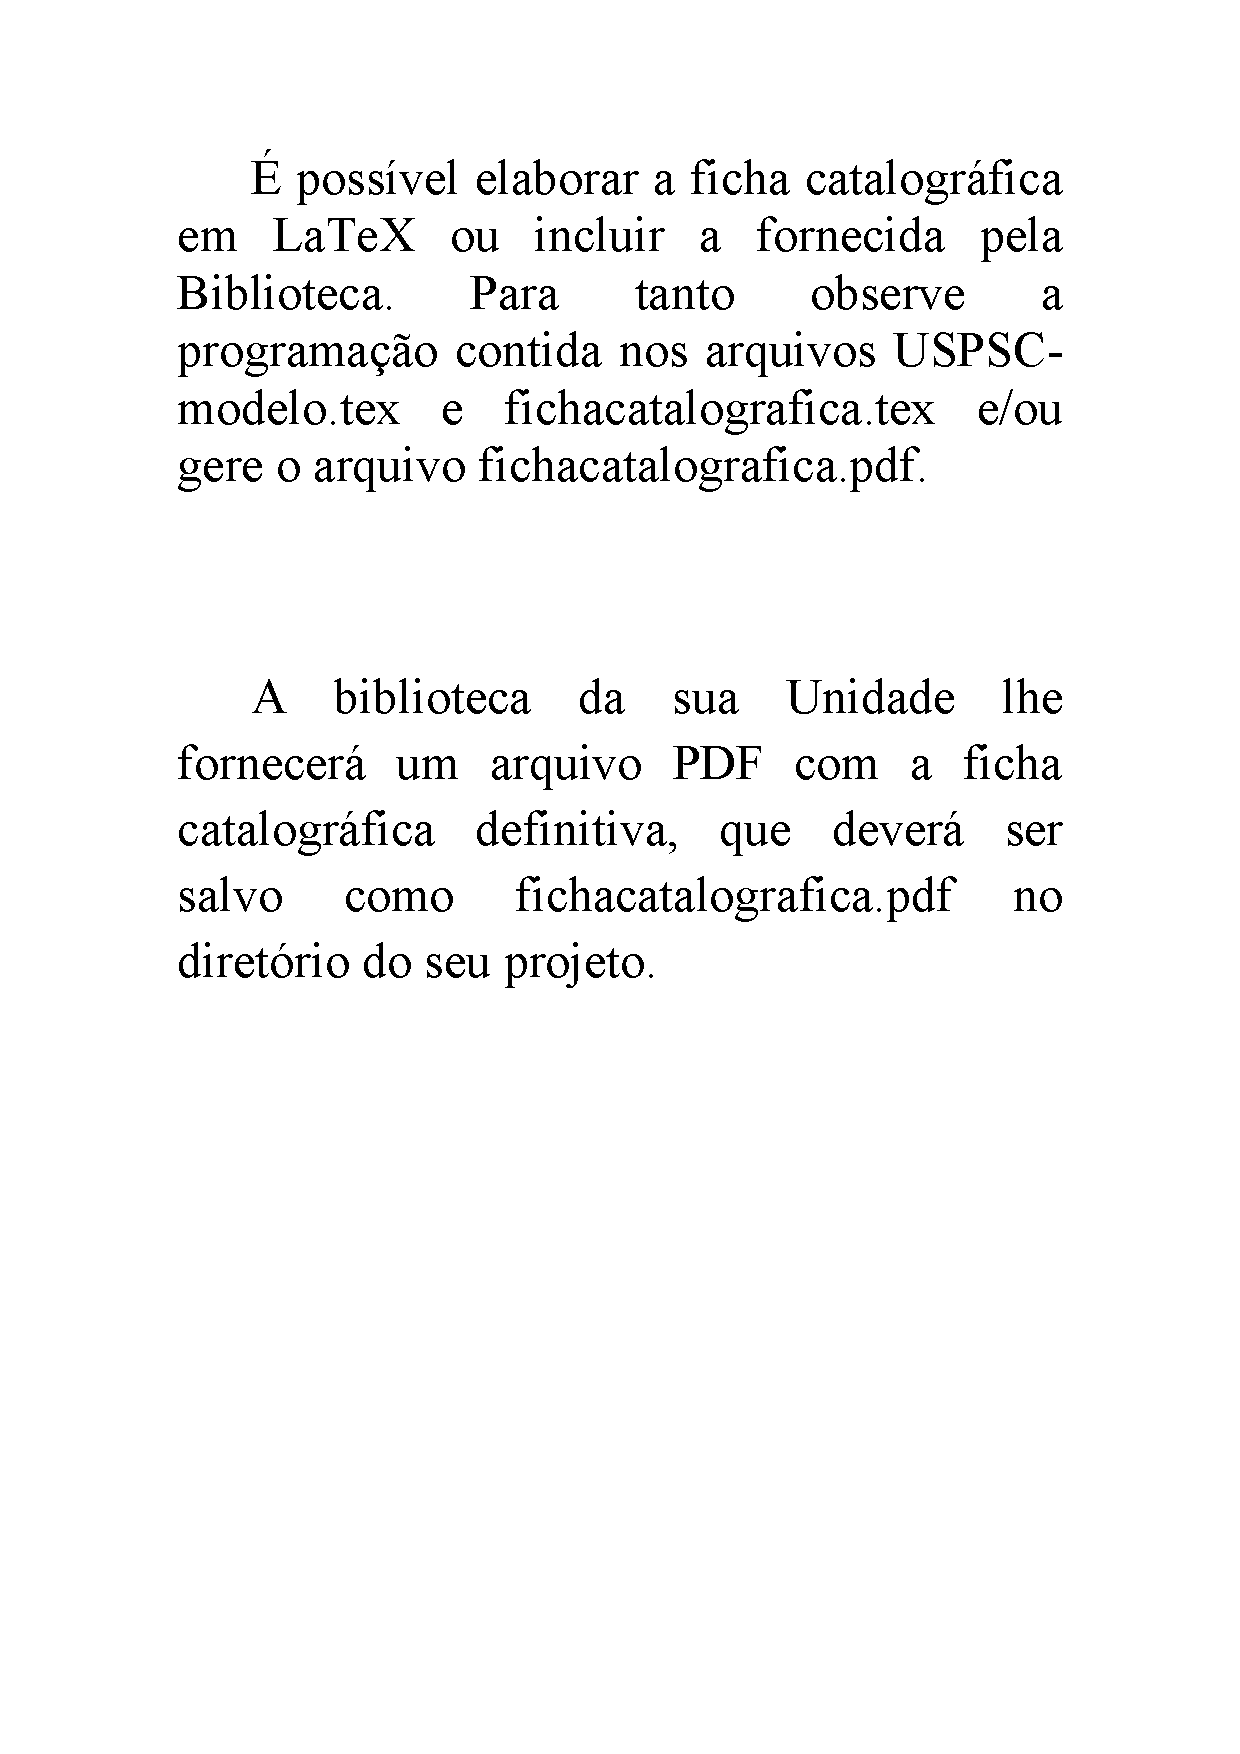
\includepdf{USPSC-TA-PreTextual/USPSC-fichacatalografica.pdf}

% Se voc\^e optar por elaborar a ficha catalogr\'afica, dever\'a 
% incluir uma % antes da linha % antes
% do comando %% USPSC-fichacatalografica.tex
% ---
% Inserir a ficha bibliografica
% ---
% Isto \'e um exemplo de Ficha Catalogr\'afica, ou ``Dados internacionais de
% cataloga\c{c}\~ao-na-publica\c{c}\~ao''. Voc\^e pode utilizar este modelo como refer\^encia. 
% Por\'em, provavelmente a biblioteca da sua universidade lhe fornecer\'a um PDF
% com a ficha catalogr\'afica definitiva ap\'os a defesa do trabalho. Quando estiver
% com o documento, salve-o como PDF no diret\'orio do seu projeto e substitua todo
% o conte\'udo de implementa\c{c}\~ao deste arquivo pelo comando abaixo:
%
\begin{fichacatalografica}
	\hspace{-1.4cm}
	\imprimirnotaautorizacao \\ \\
	%\sffamily
	\vspace*{\fill}					% Posi\c{c}\~ao vertical
\begin{center}					% Minipage Centralizado
  \imprimirnotabib \\
  \begin{table}[htb]
	\scriptsize
	\centering	
	\begin{tabular}{|p{0.9cm} p{8.7cm}|}
		\hline
	      & \\
		  &	  \imprimirautorficha     \\
		
		 \imprimircutter & 
							\hspace{0.4cm}\imprimirtitulo~  / ~\imprimirautor~ ;  ~\imprimirorientadorcorpoficha. -- 	\imprimirlocal, \imprimirdata.   \\
		
		  &  % Para incluir nota referente \`a vers\~ao corrigida no corpo da ficha,
			  % incluir % no in\'{\i}cio da linha acima e tirar a % do in\'{\i}cio da linha abaixo
			  %	\hspace{0.4cm} \imprimirtitulo~  / ~\imprimirautor~ ; ~\imprimirorientadorcorpoficha~- ~\imprimirnotafolharosto. -- \imprimirlocal, \imprimirdata.  \\
		
			\hspace{0.4cm}\pageref{LastPage} p. : il. (algumas color.) ; 30 cm.\\ 
		  & \\
		  & 
		    \hspace{0.4cm}\imprimirnotaficha ~--~ 
						  \imprimirunidademin, 
						  \imprimiruniversidademin, 
		                  \imprimirdata. \\ 
		  & \\                 
		   % Para incluir nota referente \`a vers\~ao corrigida em notas,
		    % incluir uma % no in\'{\i}cio da linha acima e	
		    % tirar a % do in\'{\i}cio da linha abaixo
		    % & \hspace{0.4cm}\imprimirnotafolharosto \\ 
		  & \\ 
		  & \hspace{0.4cm}1. LaTeX. 2. abnTeX. 3. Classe USPSC. 4. Editora\c{c}\~ao de texto. 5. Normaliza\c{c}\~ao da documenta\c{c}\~ao. 6. Tese. 7. Disserta\c{c}\~ao. 8. Documentos (elabora\c{c}\~ao). 9. Documentos eletr\^onicos. I. \imprimirorientadorficha. 
		   II. T\'{\i}tulo. \\
	
		     %Se houver co-orientador, inclua % antes da linha (antes de II. T\'{\i}tulo.) 
		     %          e tire a % antes do comando abaixo 
		     %III. T\'{\i}tulo. \\   
		  \hline
	\end{tabular}
  \end{table}
\end{center}
\end{fichacatalografica}
% ---

 
% e retirar o % do comando abaixo
%%% USPSC-fichacatalografica.tex
% ---
% Inserir a ficha bibliografica
% ---
% Isto \'e um exemplo de Ficha Catalogr\'afica, ou ``Dados internacionais de
% cataloga\c{c}\~ao-na-publica\c{c}\~ao''. Voc\^e pode utilizar este modelo como refer\^encia. 
% Por\'em, provavelmente a biblioteca da sua universidade lhe fornecer\'a um PDF
% com a ficha catalogr\'afica definitiva ap\'os a defesa do trabalho. Quando estiver
% com o documento, salve-o como PDF no diret\'orio do seu projeto e substitua todo
% o conte\'udo de implementa\c{c}\~ao deste arquivo pelo comando abaixo:
%
\begin{fichacatalografica}
	\hspace{-1.4cm}
	\imprimirnotaautorizacao \\ \\
	%\sffamily
	\vspace*{\fill}					% Posi\c{c}\~ao vertical
\begin{center}					% Minipage Centralizado
  \imprimirnotabib \\
  \begin{table}[htb]
	\scriptsize
	\centering	
	\begin{tabular}{|p{0.9cm} p{8.7cm}|}
		\hline
	      & \\
		  &	  \imprimirautorficha     \\
		
		 \imprimircutter & 
							\hspace{0.4cm}\imprimirtitulo~  / ~\imprimirautor~ ;  ~\imprimirorientadorcorpoficha. -- 	\imprimirlocal, \imprimirdata.   \\
		
		  &  % Para incluir nota referente \`a vers\~ao corrigida no corpo da ficha,
			  % incluir % no in\'{\i}cio da linha acima e tirar a % do in\'{\i}cio da linha abaixo
			  %	\hspace{0.4cm} \imprimirtitulo~  / ~\imprimirautor~ ; ~\imprimirorientadorcorpoficha~- ~\imprimirnotafolharosto. -- \imprimirlocal, \imprimirdata.  \\
		
			\hspace{0.4cm}\pageref{LastPage} p. : il. (algumas color.) ; 30 cm.\\ 
		  & \\
		  & 
		    \hspace{0.4cm}\imprimirnotaficha ~--~ 
						  \imprimirunidademin, 
						  \imprimiruniversidademin, 
		                  \imprimirdata. \\ 
		  & \\                 
		   % Para incluir nota referente \`a vers\~ao corrigida em notas,
		    % incluir uma % no in\'{\i}cio da linha acima e	
		    % tirar a % do in\'{\i}cio da linha abaixo
		    % & \hspace{0.4cm}\imprimirnotafolharosto \\ 
		  & \\ 
		  & \hspace{0.4cm}1. LaTeX. 2. abnTeX. 3. Classe USPSC. 4. Editora\c{c}\~ao de texto. 5. Normaliza\c{c}\~ao da documenta\c{c}\~ao. 6. Tese. 7. Disserta\c{c}\~ao. 8. Documentos (elabora\c{c}\~ao). 9. Documentos eletr\^onicos. I. \imprimirorientadorficha. 
		   II. T\'{\i}tulo. \\
	
		     %Se houver co-orientador, inclua % antes da linha (antes de II. T\'{\i}tulo.) 
		     %          e tire a % antes do comando abaixo 
		     %III. T\'{\i}tulo. \\   
		  \hline
	\end{tabular}
  \end{table}
\end{center}
\end{fichacatalografica}
% ---


% As informa\c{c}\~oes que comp\~oem a ficha catalogr\'afica est\~ao 
% definidas no arquivo USPSC-pre-textual-UUUU.tex
% ---

% ---
% Folha de rosto adicional
% Para imprimir a folha de rosto adicional, exigida por algumas Unidades, a exemplo do ICMC,
% retire a % antes do comando abaixo

\imprimirfolhaderostoadic*

% ---


% ---
% Inserir errata
% ---

%% USPSC-Errata.tex
\begin{errata}
	%\OnehalfSpacing 			
	A errata é um elemento opcional, que consiste de uma lista de erros da obra, precedidos pelas folhas e linhas onde eles ocorrem e seguidos pelas correções correspondentes. Deve ser inserida logo após a folha de rosto e conter a referência do trabalho para facilitar sua identificação, conforme a ABNT NBR 14724 \cite{nbr14724}.
	
	Modelo de Errata:
		
	\begin{flushleft} 
			\setlength{\absparsep}{0pt} % ajusta o espaçamento da referência	
			\SingleSpacing 
			\imprimirautorabr~ ~\textbf{\imprimirtituloresumo}.	\imprimirdata. \pageref{LastPage}p. 
			%Substitua p. por f. quando utilizar oneside em \documentclass
			%\pageref{LastPage}f.
			\imprimirtipotrabalho~-~\imprimirinstituicao, \imprimirlocal, \imprimirdata. 
 	\end{flushleft}
\vspace{\onelineskip}
\OnehalfSpacing 
\center
\textbf{ERRATA}
\vspace{\onelineskip}
\OnehalfSpacing 
\begin{table}[htb]
	\center
	\footnotesize
	\begin{tabular}{p{2cm} p{2cm} p{4cm} p{4cm} }
		\hline
		\textbf{Folha} & \textbf{Linha}  & \textbf{Onde se lê}  & \textbf{Leia-se}  \\
			\hline
			1 & 10 & auto-conclavo & autoconclavo\\
		\hline
	\end{tabular}
\end{table}
\end{errata}
% ---

% ---

% ---
% Inserir folha de aprova\c{c}\~ao
% ---

% A Folha de aprova\c{c}\~ao \'e um elemento obrigat\'orio da NBR 4724/2011 (se\c{c}\~ao 4.2.1.3). 
% Ap\'os a defesa/aprova\c{c}\~ao do trabalho, gere o arquivo folhadeaprovacao.pdf da p\'agina assinada pela banca 
% e iclua o arquivo utilizando o comando abaixo:
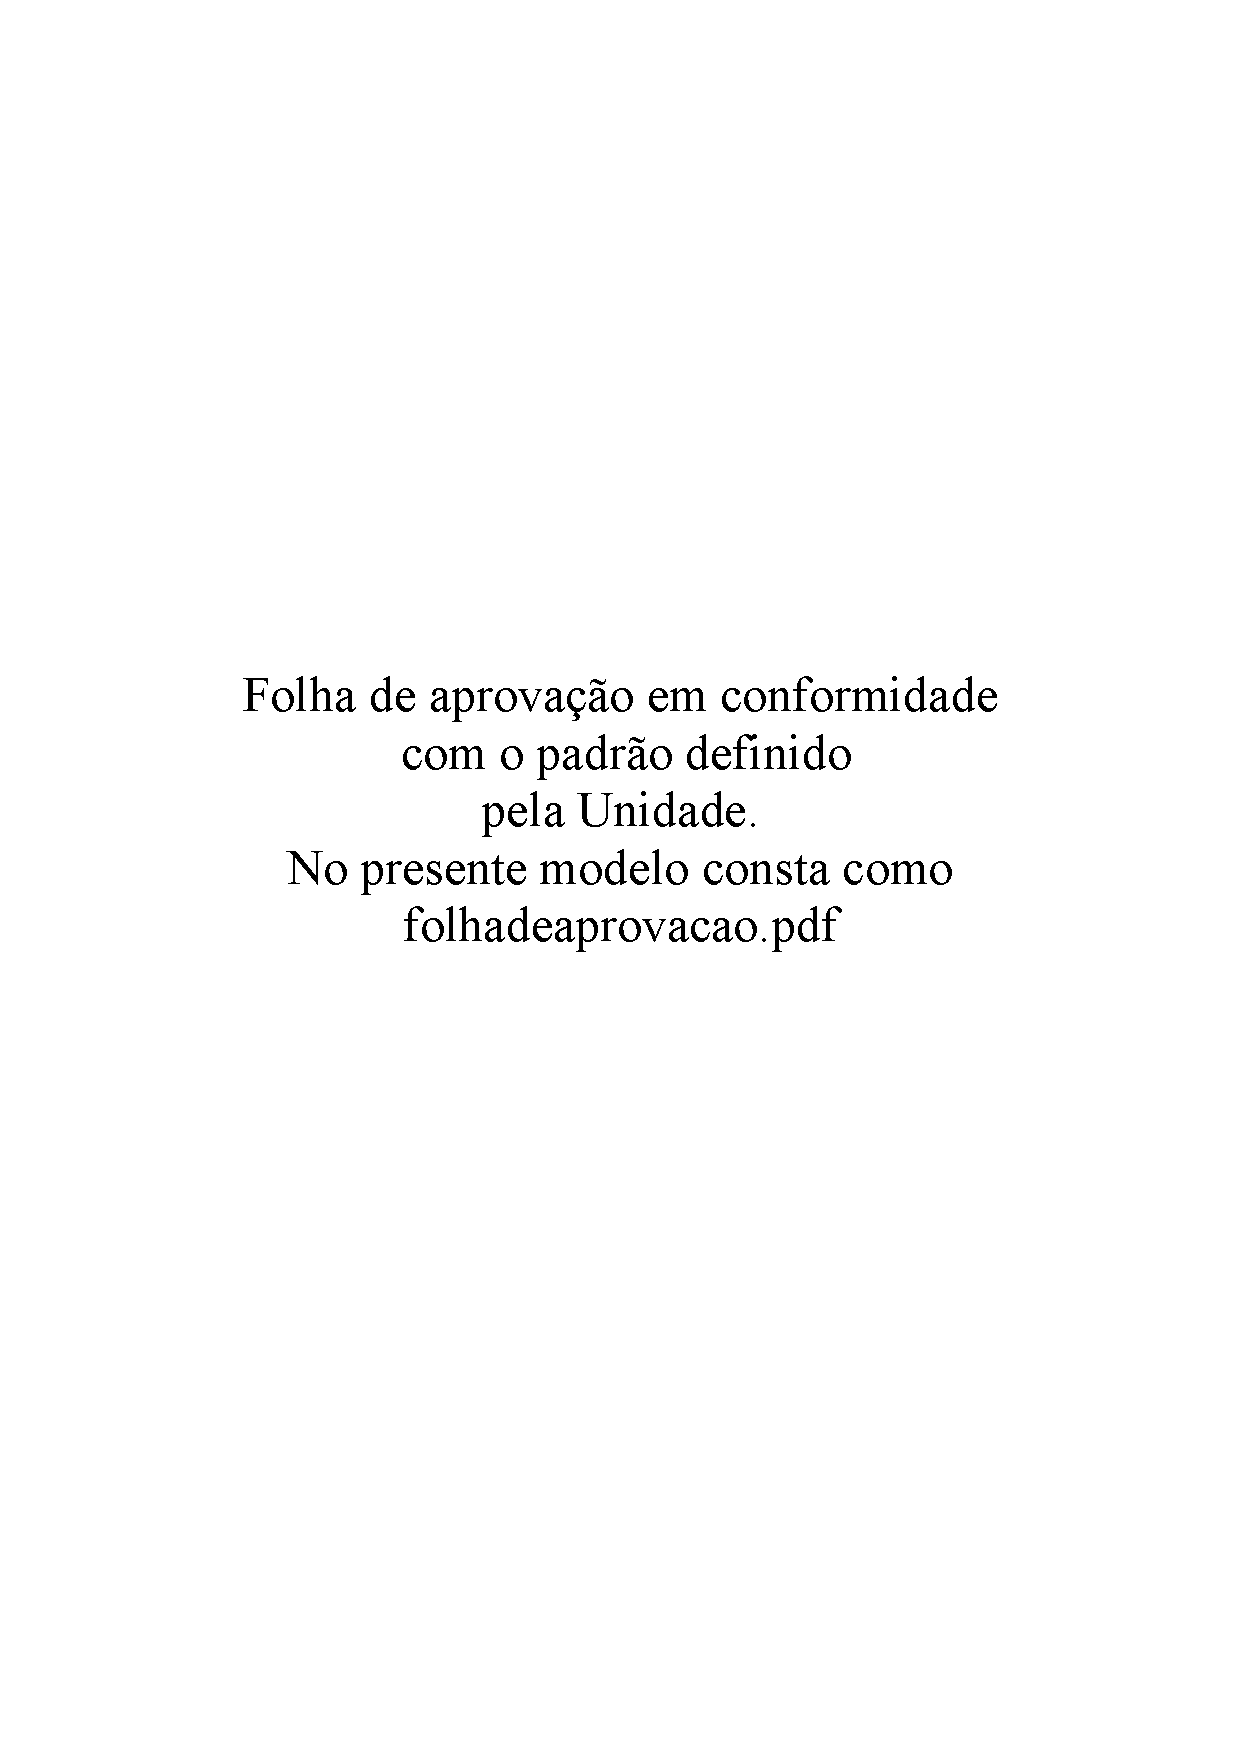
\includepdf{USPSC-TA-PreTextual/USPSC-folhadeaprovacao.pdf}
% Alternativa para a Folha de Aprova\c{c}\~ao:
% Se for a sua op\c{c}\~ao elaborar uma folha de aprova\c{c}\~ao, insira uma % antes do comando acima que inclui o arquivo folhadeaprovacao.pdf,
% tire o % do comando abaixo e altere o arquivo folhadeaprovacao.tex conforme suas necessidades
%\include{folhadeaprovacao}

\includepdf{USPSC-TA-PreTextual/USPSC-PaginaEmBranco.pdf}

% ---
% Dedicat\'oria
% ---
%% USPSC-Dedicatoria.tex
\begin{dedicatoria}
   \vspace*{\fill}
   \centering
   \noindent\textit{@[dedicatoria]@} \vspace*{\fill}
\end{dedicatoria}
% ---
% ---

% ---
% Agradecimentos
% ---
%% USPSC-Agradecimentos.tex
\begin{agradecimentos}
Quero expressar minha gratid\~ao \`as crian\c{c}as e aos jovens; que passaram pelo WASH; que est\~ao conosco e que ser\~ao o futuro do Programa.
Em especial, agrade\c{c}o a uma “crian\c{c}a sempre viva”, ativa, presente, curiosa e que outrora usou o LOGO, gostou de fazer seu jogo e trouxe essa experi\^encia para o seu mundo adulto de cientista, professor, pesquisador, gestor, amigo e companheiro de luta, h\'a mais de uma d\'ecada. Refiro-me ao Dr. Victor Pellegrini Mammana, que ao vivenciar esse prazeroso experimento, quis legar a outras crian\c{c}as o \^extase das descobertas e comprovou que \'e poss\'{\i}vel somar esfor\c{c}os da sociedade civil, das unidades de pesquisa e de educa\c{c}\~ao para contribuir com os processos de aprendizagens em ci\^encia e tecnologia.
Sou, tamb\'em, grata ao meu orientador, Prof. Dr Paulo S\'ergio de Camargo Filho pela companhia e orienta\c{c}\~ao, ao Grupo de Pesquisa STEM Education; e \`a banca de avalia\c{c}\~ao, Prof. Dra. Luciane Capelo e Profº. Dr Eduardo Damasceno.
N\~ao posso deixar de mencionar a generosidade e disposi\c{c}\~ao dos professores Drs. Ala\'{\i}de Pellegrini Mammana e Carlos Mammana, que me forneceram preciosas informa\c{c}\~oes para o trabalho.
Agrade\c{c}o, carinhosamente, \`a Professora Dra. Afira Viana Ripper, por sua contribui\c{c}\~ao para a educa\c{c}\~ao cientifica no ensino fundamental; e por participar do v\'{\i}deo, que resgata essa trajet\'oria e foi parte integrante da minha pesquisa.
Algumas pessoas, tamb\'em, precisam ser destacadas, pois foram imprescind\'{\i}veis para o Programa WASH, desde as suas origens, e marcaram essa hist\'oria (precisei colocar em ordem alfab\'etica): Adriane Pinheiro da Silva, Adriana Tito, Aldo Rabelo, Alex \^Angelo, Alexandre C\^andido Paulo, Alisson Alexandre de Ara\'ujo, Aloizio Mercadante, Am\'elia Naomi, Ant\^onio Carlos dos Santos (o Tot\'o), Ant\^onio Pestana, Alexandre Motta, Ana Paula Rodrigues, Andrea Saraiva, Andrea Dias Victor, Andrea Napolitano, Angel Luis, Antonio Bezerra de Albuquerque, Benedita Aparecida Rodrigues de Freitas, Carlinhos Almeida, C\'assia Oliveira, Cec\'{\i}lia Baranauskas, Celio Turino, Mirza Maria Pellicciotta, Celso Pansera, Celso Pan, Chico Sim\~oes, C\'{\i}ntia Cinquini, Claudio Romanelli, Cleide Santos, Mariana Moura, Clotilde Diogo, Ana Carolina de Deus Soares, Daniel Sp\'ozito, Everbal de Castro, Denise  Vieira Pereira, Dilma Rousseff,  Fabiana Kitagawa, F\'abio Couto, Delma  Medeiros, Fernanda Gon\c{c}alves, Gisele Fink, N\'adia Abiel, Gl\'aucia Veloso, Guida Calixto,  Ingridy Janaina Alves, Haissa Gabriela Silva, Irma Passoni, Isabela Maria Vieira Pereira Rodrigues, Jacqueline Baumgratrz, Jaciara Rodrigues dos Santos, Jandira Maria Rodrigues de Freitas, Jos\'e Leonardo de Oliveira, Juliana Moralles Louvison, Juliana Rabelo, Kevin Martins, Layla Xavier, Leila Bomfim, Let\'{\i}cia Mizael, Lucas Gabriel Batista da Silva, Lucas Titon, Luciano Rudinik, Fernando Accorsi, Magna Gon\c{c}alves, Malu Alencar, Marcela Moreira, Marcelo Aguirre, Maria Fernandes, Michel Morandi Alencar, Nelcina Tropardi. Pedro Tourinho, Paula Ropelo, Paulo B\'ufalo, Priya Patel, Rafael de Deus Soares, Rafael Gomes da Cruz, Rafael Proc\'opio, Renan Inqu\'erito, Renata Xavier, Roberta Santana,  Sandra Lanza, Saulo Monteiro, Sebastian Marques, Tayssa Santana,  S\'ergio Benassi, S\'{\i}lvio Ant\^onio Damasceno, S\'{\i}lvio Aparecido Spinella, TC ( Antonio Carlos), Thatiane Verni Lopes de Ara\'ujo, Toni Klaus, Valdirene Maria dos Santos, Vitor de Oliveira Pochmann, Wagner Rodrigo Silva, Wil Namen, dentre tantos outros.
A todas as gera\c{c}\~oes do WASH: as que passaram, as que compartilham conosco, nesse ano de 2023, os 10 anos do Programa: s\~ao colegas, bolsistas, educandos, educadores, cientistas, coordenadores, orientadores, Conselhos de classes, Sindicatos, gestores, pesquisadores, vereadores, comunidades, os entes federados, que acreditam na ci\^encia e no papel transformador da educa\c{c}\~ao.
Meus agradecimentos, tamb\'em. \`as institui\c{c}\~oes parceiras: Conselho Nacional de Desenvolvimento Cient\'{\i}fico e Tecnol\'ogico - CNPq , Funda\c{c}\~ao Arauc\'aria, WASH Paran\'a, Cia Bola de Meia, Legislativo Federal, por meio dos deputados: Ivan Valente, Alex e Luiza Canziani, Alexandre Padilha, Vicentinho, Carlos Zaratini, Orlando Silva e Alexandre Cury, que foram sens\'{\i}veis e valorizaram a educa\c{c}\~ao cientifica, atrav\'es do Programa WASH. Aos legislativos de Prado Ferreira e Dr. Camargo por fazerem o WASH leis municipais. N\~ao posso deixar de reconhecer a contribui\c{c}\~ao da AkiPosso , com o apoio dos colegas Kevin Martins, Adriana Tito, Priya Patel, Caroline Gardemann, Nelcina Tropardi e Daniela Napolitano. Por fim, agrade\c{c}o a minha fam\'{\i}lia, a minha filha, Agatha Abayomi Silva Sene, aos meus pais, Maria Imaculada de Oliveira e Silva e Joaquim Roberto da Silva, ao meu irm\~ao Eduardo Roberto da Silva in memoriam - presente! e ao Alessandro, que contribu\'{\i}ram para que as condi\c{c}\~oes necess\'arias para o desenvolvimento dessa pesquisa fossem as mais leves para a execu\c{c}\~ao do meu estudo.
Termino enfatizando os papeis especiais do Vereador Paulo Bufalo, que est\'a nesta caminhada conosco desde os prim\'ordios do programa, e da Dra. Andrea Dias Victor, servidora do CNPq que permanece aceitando, com compromisso p\'ublico, excel\^encia administrativa e acad\^emica, a carga de gest\~ao do programa WASH, representada por centenas de bolsistas semestrais.
% @[pontoinsercaoparagrafoagradecimento]@

\end{agradecimentos}
% ---
% ---

% ---
% Ep\'{\i}grafe
% ---
%% USPSC-Epigrafe.tex
\begin{epigrafe}
    \vspace*{\fill}
	\begin{flushright}\textit{. Brasil Meu Brasil ande pra frente. Venha com a gente pra Avenida desfilar . \'E chegada a hora da verdade. N\~ao \'e preciso mais voc\^e se disfar\c{c}ar. Levante os panos, mostra tua cara. E assuma essa cara que voc\^e tem. Brasil Terra dos Ianom\^amis. Essas matas s\~ao de Oxossi. Deixa na terra as riquezas de Oxum. Devolva pro povo o que \'e do povo. Bote os malditos pra fora. E vamos refazer essa na\c{c}\~ao. Pois,o pa\'{i}s que  \'e o olho d’\'agua do mundo n\~ao pode ver sofrer. N\~ao pode ver chorar um povo que trabalha, canta e \'e feliz. Chega de tanta injusti\c{c}a, chega de corrup\c{c}\~ao. Vamos arrumar a casa, vamos dividir o nosso ch\~ao. E chega de sofrer e chega de chorar. Oh p\'atria amada idolatrada. Salve-se Brasil! Antonio Carlos (TC) Santos Silva Alu\'{i}zio Jeremias (Samba Enredo, 1988)}
	\end{flushright}
\end{epigrafe}
% ---
% ---

% A T E N \c{C} \~A O
% Se o idioma do texto for em ingl\^es, o abstract deve preceder o resumo
% resumo em portugu\^es
%
% Resumo
% ---
%% USPSC-Resumo.tex
\setlength{\absparsep}{18pt} % ajusta o espa\c{c}amento dos par\'agrafos do resumo
\begin{resumo}
\begin{flushleft} 
\setlength{\absparsep}{0pt} % ajusta o espa\c{c}amento da refer\^encia
\SingleSpacing 
\imprimirautorabr~~\textbf{\imprimirtituloresumo}.\imprimirdata. \pageref{LastPage}p. 
%Substitua p. por f. quando utilizar oneside em \documentclass
%\pageref{LastPage}f.
\imprimirtipotrabalho~-~\imprimirinstituicao, \imprimirlocal, \imprimirdata. 
 \end{flushleft}
\OnehalfSpacing 
O  Programa Workshop de Aficcionados em Software e Hardware (WASH), de educa\c{c}\~ao em Ci\^encia, Tecnologia, Engenharia, Artes e Matem\'atica (STEAM) \'e executado desde 2013 em dezenas de munic\'{\i}pios brasileiros e com milhares de crian\c{c}as atendidas. Ap\'os anos de pr\'atica, as caracter\'{\i}sticas principais foram agrupadas no Documento de Refer\^encia publicado em 2018, anexado \`a Portaria CTI 178/2018. Esta pesquisa \'e dividida em 2 eixos: m\'etodo historiogr\'afico (eixo 1) e o emprego de consultas estruturadas a uma base de dados especialmente desenvolvida para produzir os indicadores (eixo 2). O trabalho buscou comparar, a partir das defini\c{c}\~oes do Documento de Refer\^encia, \textquotedbl\{\}o que o WASH gostaria de ter sido\textquotedbl\{\} com \textquotedbl\{\}o que o WASH conseguiu ser\textquotedbl\{\}, informa\c{c}\~ao decorrente dos Resultados e An\'alise desta disserta\c{c}\~ao. Para objetivar essa compara\c{c}\~ao, foram formuladas seis hip\'oteses, a partir do Documento de Refer\^encia, que ao final do trabalho foram submetidas a uma valida\c{c}\~ao.  A an\'alise dos sucessos e insucessos dessa valida\c{c}\~ao permitiu produzir uma revis\~ao do Documento de Refer\^encia, a qual \'e o principal produto educacional desta disserta\c{c}\~ao, quesito obrigat\'orio para a obten\c{c}\~ao do t\'{\i}tulo em Mestrado. Agrega-se a esse produto educacional a entrevista com a Profa. Afira Ripper, um dos elementos usados para a an\'alise no eixo 1 e, tamb\'em, um testemunho bastante raro sobre a vinda de Seymour Papert ao Brasil no final do s\'eculo passado.
% @[pontoinsercaoparagraforesumo]@
 

 \textbf{Palavras-chave}: Papert, STEAM, STEM, WASH
\end{resumo}
% ---

% Abstract
% ---
%% USPSC-Abstract.tex
%\autor{Silva, M. J.}
\begin{resumo}[Abstract]
 \begin{otherlanguage*}{english}
	\begin{flushleft} 
		\setlength{\absparsep}{0pt} % ajusta o espaçamento dos par\'agrafos do resumo		
 		\SingleSpacing  		\imprimirautorabr~~\textbf{\imprimirtitleabstract}.	\imprimirdata.  \pageref{LastPage}p. 
		%Substitua p. por f. quando utilizar oneside em \documentclass
		%\pageref{LastPage}f.
		\imprimirtipotrabalhoabs~-~\imprimirinstituicao, \imprimirlocal, 	\imprimirdata. 
 	\end{flushleft}
	\OnehalfSpacing 
   This is the english abstract.

   \vspace{\onelineskip}
 
   \noindent 
   \textbf{Keywords}: LaTeX. USPSC class. Thesis. Dissertation. Conclusion course paper. 
 \end{otherlanguage*}
\end{resumo}

% ---

% ---
% inserir lista de figurass
% ---
\pdfbookmark[0]{\listfigurename}{lof}
\listoffigures*
\cleardoublepage
% ---

% ---
% inserir lista de tabelas
% ---
\pdfbookmark[0]{\listtablename}{lot}
\listoftables*
\cleardoublepage
% ---

% ---
% inserir lista de quadros
% ---
\pdfbookmark[0]{\listofquadroname}{loq}
\listofquadro*
\cleardoublepage
% ---

% ---
% inserir lista de abreviaturas e siglas
% ---
% USPSC-AbreviaturasSiglas.tex
\begin{siglas}
    \item[ABNT] Associação Brasileira de Normas Técnicas
    \item[abnTeX] ABsurdas Normas para TeX
	\item[IBGE] Instituto Brasileiro de Geografia e Estatística
	\item[LaTeX] Lamport TeX
	\item[USP] Universidade de São Paulo
	\item[USPSC] Campus USP de São Carlos
\end{siglas}

% ---

% ---
% inserir lista de s\'{\i}mbolos
% ---
% USPSC-Simbolos.tex
\begin{simbolos}
  \item[$ \Gamma $] Letra grega Gama
  \item[$ \Lambda $] Lambda
  \item[$ \zeta $] Letra grega minúscula zeta
  \item[$ \in $] Pertence
\end{simbolos}
% ---
% ---
% inserir o sumario
% ---
\pdfbookmark[0]{\contentsname}{toc}
\tableofcontents*
\cleardoublepage
% ---
% ----------------------------------------------------------
% ELEMENTOS TEXTUAIS
% ----------------------------------------------------------
\textual
% Os cap\'{\i}tulos s\~ao inseridos como arquivos externos 

% Cap\'{\i}tulo 1 - Introdu\c{c}\~ao
% ---
\chapter[ESTRUTURA DO TEXTO]{ESTRUTURA DO TEXTO}\label{ESTRUTURA DO TEXTO}
Este trabalho busca utilizar a forma mais can\^onica de estrutura\c{c}\~ao de um texto cient\'{\i}fico [XXX Oftalmo DOI: 10.5935/0034-7280.20140055]:








\begin{alineas}
\item introdu\c{c}\~ao
\item m\'etodos
\item resultados
\item discuss\~ao
\end{alineas}

A refer\^encia [XXX Oftalmo DOI: 10.5935/0034-7280.20140055] busca identificar o car\'ater principal de cada um dos elementos acima por meio de uma pergunta, como segue:








\begin{alineas}
\item Introdu\c{c}\~ao - que pergunta foi feita?
\item M\'etodos - como ela foi estudada?
\item Resultados - o que foi achado?
\item Discuss\~ao - o que estes achados significam? 
\end{alineas}

\begin{flushright}
\setlength{\absparsep}{0pt}
\tiny \begin{flushright}
\setlength{\absparsep}{0pt}
\tiny \begin{flushright}
\setlength{\absparsep}{0pt}
\tiny \begin{flushright}
\setlength{\absparsep}{0pt}
\tiny \begin{flushright}
\setlength{\absparsep}{0pt}
\tiny \begin{flushright}
\setlength{\absparsep}{0pt}
\tiny \begin{flushright}
\setlength{\absparsep}{0pt}
\tiny (fonte: [XXX Oftalmo DOI: 10.5935/0034-7280.20140055]:) \normalsize 
\end{flushright}

 \normalsize 
\end{flushright}

 \normalsize 
\end{flushright}

 \normalsize 
\end{flushright}

 \normalsize 
\end{flushright}

 \normalsize 
\end{flushright}

 \normalsize 
\end{flushright}


Uma forma diferente de expressar esses mesmos conceitos \'e atribuir a pergunta "por que fiz? \`a Introdu\c{c}\~ao, atribuir a pergunta "como fiz? aos M\'etodos e atribuir a pergunta "o que obtive? aos Resultados, de forma que a pesquisa empregada permita observar o mesmo objeto em estudo por meio de 3 dimens\~oes que se complementam. 







A estrutura indicada acima pode ter variantes mais completas como a descrita em [XXX How to Write a Paper in Scientific Journal Style and Format]:








\begin{alineas}
\item Resumo - O que eu fiz de uma forma bem sint\'etica ("in a nutshell)?
\item Introdu\c{c}\~ao - Qual \'e o problema?
\item Materiais e M\'etodos - Como eu resolvi o problema?
\item Resultados - O que eu achei?
\item Agradecimentos (opcional) - Quem me ajudou a fazer?
\item Literatura citada - Quais trabalhos eu usei como refer\^encia?
\item Ap\^endices - Informa\c{c}\~ao Extra
\end{alineas}

\begin{flushright}
\setlength{\absparsep}{0pt}
\tiny \begin{flushright}
\setlength{\absparsep}{0pt}
\tiny \begin{flushright}
\setlength{\absparsep}{0pt}
\tiny \begin{flushright}
\setlength{\absparsep}{0pt}
\tiny \begin{flushright}
\setlength{\absparsep}{0pt}
\tiny \begin{flushright}
\setlength{\absparsep}{0pt}
\tiny \begin{flushright}
\setlength{\absparsep}{0pt}
\tiny (tradu\c{c}\~ao livre de [XXX How to Write a Paper in Scientific Journal Style and Format]) \normalsize 
\end{flushright}

 \normalsize 
\end{flushright}

 \normalsize 
\end{flushright}

 \normalsize 
\end{flushright}

 \normalsize 
\end{flushright}

 \normalsize 
\end{flushright}

 \normalsize 
\end{flushright}


A variante acima, embora voltada para publica\c{c}\~oes curtas, \'e v\'alida para outros tipos de registros cient\'{\i}ficos e tamb\'em \'e baseada na ideia das 3 dimens\~oes descrita acima: "por que?, "como? e "o que?. 







De forma mais completa ainda, mas com a mesma estrutura b\'asica: 







\begin{flushright}
\setlength{\absparsep}{0pt}
\tiny \begin{flushright}
\setlength{\absparsep}{0pt}
\tiny \begin{flushright}
\setlength{\absparsep}{0pt}
\tiny \begin{flushright}
\setlength{\absparsep}{0pt}
\tiny \begin{flushright}
\setlength{\absparsep}{0pt}
\tiny \begin{flushright}
\setlength{\absparsep}{0pt}
\tiny \begin{flushright}
\setlength{\absparsep}{0pt}
\tiny MEO 2018 \normalsize 
\end{flushright}

 \normalsize 
\end{flushright}

 \normalsize 
\end{flushright}

 \normalsize 
\end{flushright}

 \normalsize 
\end{flushright}

 \normalsize 
\end{flushright}

 \normalsize 
\end{flushright}




\begin{figure}[htb]

	\begin{center}

		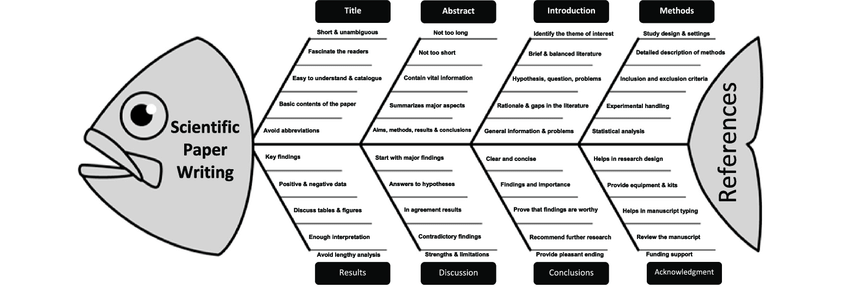
\includegraphics[scale=0.5]{../../imagens/MEOS-Fish-Bone-Model-Basic-components-of-a-scientific-paper.png}

	\end{center}

	\caption{\label{MEOS-Fish-Bone-Model-Basic-components-of-a-scientific-paper}@[caption-MEOS-Fish-Bone-Model-Basic-components-of-a-scientific-paper]@}

	\legend{Fonte: \citeonline{cite-MEOS-Fish-Bone-Model-Basic-components-of-a-scientific-paper}}

\end{figure}
Uma vez que a Fig. 1 \'e um pouco "congestionada no sentido da densidade de informa\c{c}\~oes apresentadas, cabe uma descri\c{c}\~ao de cada "costela da espinha-de-peixe de MEOs, transcrita aqui na forma de uma tabela:







/var/www/html/tese/dados/tabelas/tabela\_estrutura\_de\_texto.html
As 3 estruturas exemplificadas [XXX MEO, How to Write e Oftalmo] acima tratam, principalmente, de papers cient\'{\i}ficos, em que a concis\~ao \'e especialmente necess\'aria. Mas papers cientificos n\~ao s\~ao o \'unico formato dispon\'{\i}vel para realizar uma comunica\c{c}\~ao cient\'{\i}fica. 







Existem formatos mais extensos para documenta\c{c}\~ao, tais como: relat\'orios, teses, comunica\c{c}\~oes r\'apidas. Alaide Mammana tamb\'em explora estas nuances, muito embora a estrutura b\'asica seja sempre "Introdu\c{c}\~ao, M\'etodos, Resultados e Discuss\~ao, como j\'a refor\c{c}ado aqui.







\begin{flushright}
\setlength{\absparsep}{0pt}
\tiny \begin{flushright}
\setlength{\absparsep}{0pt}
\tiny \begin{flushright}
\setlength{\absparsep}{0pt}
\tiny \begin{flushright}
\setlength{\absparsep}{0pt}
\tiny \begin{flushright}
\setlength{\absparsep}{0pt}
\tiny \begin{flushright}
\setlength{\absparsep}{0pt}
\tiny \begin{flushright}
\setlength{\absparsep}{0pt}
\tiny [XXX Alaide Mammana, Documenta\c{c}\~ao cient\'{\i}ficas] \normalsize 
\end{flushright}

 \normalsize 
\end{flushright}

 \normalsize 
\end{flushright}

 \normalsize 
\end{flushright}

 \normalsize 
\end{flushright}

 \normalsize 
\end{flushright}

 \normalsize 
\end{flushright}


O presente texto, por se tratar de uma disserta\c{c}\~ao, pode se valer desses formatos mais extensos, uma vez que se trata da "defesa para obten\c{c}\~ao de um t\'{\i}tulo (mestrado), em que a presente candidata tem que demonstrar erudi\c{c}\~ao nos temas abordados. O formato menos conciso permite \`a esta candidata expor melhor a sua busca por uma erudi\c{c}\~ao, dado que comporta a revis\~ao de conhecimentos j\'a existentes de forma mais estendida.







\section[Descri\c{c}\~ao da Introdu\c{c}\~ao]{Descri\c{c}\~ao da Introdu\c{c}\~ao}\label{Descri\c{c}\~ao da Introdu\c{c}\~ao}
Seguindo as sugest\~oes presentes em S. MEO, optou-se por uma introdu\c{c}\~ao curta, leve e objetiva. A introdu\c{c}\~ao \'e estruturada para culminar, por meio de seus \'ultimos par\'agrafos, na descri\c{c}\~ao do objeto de estudo. O caminho percorrido \'e o de descrever esse objeto do mais geral at\'e o espec\'{\i}fico. 







\begin{flushright}
\setlength{\absparsep}{0pt}
\tiny \begin{flushright}
\setlength{\absparsep}{0pt}
\tiny \begin{flushright}
\setlength{\absparsep}{0pt}
\tiny \begin{flushright}
\setlength{\absparsep}{0pt}
\tiny \begin{flushright}
\setlength{\absparsep}{0pt}
\tiny \begin{flushright}
\setlength{\absparsep}{0pt}
\tiny \begin{flushright}
\setlength{\absparsep}{0pt}
\tiny [citar XXX] \normalsize 
\end{flushright}

 \normalsize 
\end{flushright}

 \normalsize 
\end{flushright}

 \normalsize 
\end{flushright}

 \normalsize 
\end{flushright}

 \normalsize 
\end{flushright}

 \normalsize 
\end{flushright}


Para que que pudesse se expressar de forma organizada, buscando demonstrar sua erudi\c{c}\~ao, sem perder a objetividade da "Introdu\c{c}\~ao", a presente candidata acatou a sugest\~ao do orientador de incluir um cap\'{\i}tulo de "Fundamenta\c{c}\~ao Te\'orica, no qual os temas pincelados na "Introdu\c{c}\~ao pudessem ser mais profundamente descritos, sem preju\'{\i}zo para um formato "leve e balanceado para a apresenta\c{c}\~ao da literatura na introdu\c{c}\~ao, um aspecto que, segundo S.A. Meo, e.g., deve ser perseguido pelo redator de textos cient\'{\i}ficos. Assim, a exposi\c{c}\~ao na "Introdu\c{c}\~ao busca ser o mais sint\'etica poss\'{\i}vel, com direcionamento para a "Fundamenta\c{c}\~ao Te\'orica sempre que for necess\'ario aprofundar em algum conceito. 







Para facilitar a leitura, a presente candidata optou, tamb\'em, por colocar em subse\c{c}\~oes da "Introdu\c{c}\~ao a exposi\c{c}\~ao dos problemas, hip\'oteses, das quest\~oes e dos objetos de interesse.







\section[Descri\c{c}\~ao de Materiais e M\'etodos]{Descri\c{c}\~ao de Materiais e M\'etodos}\label{Descri\c{c}\~ao de Materiais e M\'etodos}
Uma vez que a presente pesquisa tem por objeto a caracteriza\c{c}\~ao do Projeto WASH quanto \`a sua hist\'oria (trajet\'oria), m\'etodos e resultados, a descri\c{c}\~ao do m\'etodo do WASH deve ser considerada como resultado do m\'etodo da pesquisa. Em outras palavras, uma das dimens\~oes do m\'etodo aqui empregado refere-se a caracterizar o m\'etodo do WASH. Portanto, a pesquisa se baseia num m\'etodo de caracteriza\c{c}\~ao de m\'etodos. Assim, a descri\c{c}\~ao do m\'etodo do WASH deve ser considerada uma decorr\^encia da aplica\c{c}\~ao do m\'etodo da pesquisa desta disserta\c{c}\~ao e, por esse motivo, encontra-se no cap\'{\i}tulo de "Resultados e n\~ao no cap\'{\i}tulo de "Materiais e M\'etodos. 







\section[Descricao de Resultados e Discuss\~oes]{Descricao de Resultados e Discuss\~oes}\label{Descricao de Resultados e Discuss\~oes}
A candidata optou por juntar em um \'unico cap\'{\i}tulo os resultados e as discuss\~oes ("Resultados e Discuss\~oes). Esta op\c{c}\~ao visa garantir uma melhor fluidez, dado que permite apresentar as op\c{c}\~oes de an\'alise que levaram \`a proposta de melhorias no m\'etodo do WASH, o produto final desta disserta\c{c}\~ao. 







\section[Produto Tecnol\'ogico]{Produto Tecnol\'ogico}\label{Produto Tecnol\'ogico}
A presente disserta\c{c}\~ao, por se tratar de um Mestrado Tecnol\'ogico, deve culminar com a apresenta\c{c}\~ao de um "produto de car\'ater pr\'atico, que no presente caso ser\'a uma revis\~ao do Documento de Refer\^encia do Projeto WASH  constante do anexo da  Portaria CTI 178/2018). Por esse motivo foi acrescentado \`a estrutura do documento um cap\'{\i}tulo de "Produto Tecnol\'ogico. Biblioteca Cidad\~a Paulo Freire







\chapter[INTRODU\c{C}\~AO]{INTRODU\c{C}\~AO}\label{INTRODU\c{C}\~AO}
Aos olhos de jovens observadores contempor\^aneos, parece natural a relativa desenvoltura com que as pessoas utilizam os computadores e os celulares nos dias de hoje. J\'a est\~ao bastante difundidos os servi\c{c}os de governo eletr\^onico, os sites de com\'ercio eletr\^onico, os  aplicativos de entrega, as plataformas de ensino, de reuni\~oes, a busca por  trabalho, oportunidades, voto eletr\^onico, banco e caixa eletr\^onico, por exemplo.







\begin{flushright}
\setlength{\absparsep}{0pt}
\tiny \begin{flushright}
\setlength{\absparsep}{0pt}
\tiny \begin{flushright}
\setlength{\absparsep}{0pt}
\tiny \begin{flushright}
\setlength{\absparsep}{0pt}
\tiny \begin{flushright}
\setlength{\absparsep}{0pt}
\tiny \begin{flushright}
\setlength{\absparsep}{0pt}
\tiny \begin{flushright}
\setlength{\absparsep}{0pt}
\tiny [XXX].  \normalsize 
\end{flushright}

 \normalsize 
\end{flushright}

 \normalsize 
\end{flushright}

 \normalsize 
\end{flushright}

 \normalsize 
\end{flushright}

 \normalsize 
\end{flushright}

 \normalsize 
\end{flushright}


Essas ferramentas s\~ao continuadamente revistas e melhoradas, assim como n\~ao param de se multiplicar para atender e se adaptar aos desafios impostos pela evolu\c{c}\~ao da conviv\^encia em sociedade. Um exemplo dessa necessidade de adapta\c{c}\~ao foi recentemente evidenciado pela forma como a sociedade respondeu \`as imposi\c{c}\~oes sanit\'arias relativas \`a pandemia de 2020, quando os cidad\~aos tiveram que se adaptar ao isolamento e encontrar formas para continuarem produtivos por meios das redes digitais.







\begin{flushright}
\setlength{\absparsep}{0pt}
\tiny \begin{flushright}
\setlength{\absparsep}{0pt}
\tiny \begin{flushright}
\setlength{\absparsep}{0pt}
\tiny \begin{flushright}
\setlength{\absparsep}{0pt}
\tiny \begin{flushright}
\setlength{\absparsep}{0pt}
\tiny \begin{flushright}
\setlength{\absparsep}{0pt}
\tiny \begin{flushright}
\setlength{\absparsep}{0pt}
\tiny [XXX]. \normalsize 
\end{flushright}

 \normalsize 
\end{flushright}

 \normalsize 
\end{flushright}

 \normalsize 
\end{flushright}

 \normalsize 
\end{flushright}

 \normalsize 
\end{flushright}

 \normalsize 
\end{flushright}


\'E poss\'{\i}vel afirmar que as pessoas t\^em usado com frequ\^encia e com relativa facilidade as ferramentas digitais instaladas em computadores e em celulares, sejam aplicativos de mensagens, buscadores (browsers), correio eletr\^onico, redes sociais, entre outras. Esse uso d\'a-se em v\'arios contextos: profissional, educacional, de entretenimento, de intera\c{c}\~ao social, al\'em dos servi\c{c}os de governo eletr\^onico.







As novas gera\c{c}\~oes precisam, no entanto, saber que n\~ao foi sempre assim. Muito embora a percep\c{c}\~ao corrente de que o uso de computadores e celulares \'e indispens\'avel para o conv\'{\i}vio na sociedade, a rigor seu uso \'e relativamente recente.







\'E poss\'{\i}vel identificar a evolu\c{c}\~ao das telecomunica\c{c}\~oes a partir do s\'eculo passado como origem das transforma\c{c}\~oes tecnol\'ogicas que disponibilizaram tecnologias digitais em larga escala. Esse fato foi identificado, por exemplo, por PIERRE LEVY, em Cibercultura, 







durante uma entrevista nos anos 50, Albert Einstein (1879-1955) declarou que tr\^es grandes bombas haviam  explodido durante o s\'eculo XX: a bomba demogr\'afica, a bomba at\^omica e a bomba das telecomunica\c{c}\~oes. Esta \'ultima ‘bomba’ foi chamada por Roy Ascott ( pioneiro e te\'orico das artes em rede) de Segundo Dil\'uvio, o das informa\c{c}\~oes. As telecomunica\c{c}\~oes geram esse novo dil\'uvio por conta da natureza exponencial, explosiva e ca\'otica do seu crescimento. A quantidade de dados e links se multiplica, acelera, aumento de links, banco de dados, hipertextos nas redes, contos transversais, etc.
\begin{flushright}
\setlength{\absparsep}{0pt}
\tiny \begin{flushright}
\setlength{\absparsep}{0pt}
\tiny \begin{flushright}
\setlength{\absparsep}{0pt}
\tiny \begin{flushright}
\setlength{\absparsep}{0pt}
\tiny \begin{flushright}
\setlength{\absparsep}{0pt}
\tiny \begin{flushright}
\setlength{\absparsep}{0pt}
\tiny \begin{flushright}
\setlength{\absparsep}{0pt}
\tiny [1] \normalsize 
\end{flushright}

 \normalsize 
\end{flushright}

 \normalsize 
\end{flushright}

 \normalsize 
\end{flushright}

 \normalsize 
\end{flushright}

 \normalsize 
\end{flushright}

 \normalsize 
\end{flushright}


Ainda, segundo Pierre Levy,







"O segundo dil\'uvio n\~ao ter\'a fim. N\~ao h\'a nenhum fundo s\'olido sob o oceano de informa\c{c}\~oes. Devemos aceit\'a-lo como nossa nova condi\c{c}\~ao. Temos que ensinar nossos filhos a nadar, a flutuar, talvez a navegar.
Para desenvolver e dar acesso a estes recursos tecnol\'ogicos,  governos tiveram que prover a infraestrutura de ci\^encia e tecnologia, comunica\c{c}\~oes e de redes digitais e os meios de acesso a essas redes, algumas vezes com a participa\c{c}\~ao da iniciativa privada. Na outra ponta, tiveram que promover projetos, formular pol\'{\i}ticas p\'ublicas de C\&T para o desenvolvimento e  dissemina\c{c}\~ao do uso das tecnologias da informa\c{c}\~ao e comunica\c{c}\~ao e para a capacita\c{c}\~ao dos cidad\~aos atrav\'es de programas de car\'ater educacional e de forma\c{c}\~ao profissional. No Brasil, a g\^enese desse esfor\c{c}o foi deflagrada pelo Estado no in\'{\i}cio da d\'ecada de 60 [2], sendo que suas a\c{c}\~oes perduram at\'e os dias de hoje. Uma revis\~ao essa trajet\'oria brasileira ser\'a apresentada no cap\'{\i}tulo de "Fundamenta\c{c}\~ao Te\'orica.







Se para alguns as redes digitais tinham o objetivo de atender os indiv\'{\i}duos em suas necessidade de relacionamento com o governo, afinal a pr\'opria internet nasceu no contexto governamental [XXX], elas foram mais longe, e alcan\c{c}aram todas as demais dimens\~oes do cidad\~ao, tais como: consumidor, benefici\'ario de servi\c{c}os de sa\'ude, educando, trabalhador, empreendedor, contribuinte, eleitor, entre outras.  Essa expans\~ao se deu como resultado de v\'arias a\c{c}\~oes, mas sua universaliza\c{c}\~ao foi resultado principalmente do surgimento de novas formas de relacionamento social representadas pelas redes sociais digitais, que tornaram mais acess\'{\i}veis novas ferramentas de apoio ao ensino em sala de aula, o ensino \`a dist\^ancia, o com\'ercio eletr\^onico, a elei\c{c}\~ao eletr\^onica, os "market-places, os aplicativos de transporte, etc. 







Estas transforma\c{c}\~oes tiveram impactos econ\^omicos e sociais profundos, inclusive nas rela\c{c}\~oes de trabalho, seja na cria\c{c}\~ao ou extin\c{c}\~ao de posto de trabalho, bem como em suas formas de contrata\c{c}\~ao, jornada, remunera\c{c}\~ao, inclusive com a precariza\c{c}\~ao dos direitos trabalhistas. Elas est\~ao muito bem descritas  no relat\'orio da Unesco  de 2004 "Social Transformation in an Information Society: Rethinking Access to You and the World [3]. A amplitude destas  transforma\c{c}\~oes por que passa a sociedade humana \'e sintetizada no que se chama  Sociedade da Informa\c{c}\~ao ou  Era Digital ou Era da Informa\c{c}\~ao. Uma breve revis\~ao sobre esse conceito  \'e apresentada na fundamenta\c{c}\~ao te\'orica. 







O efeito destas transforma\c{c}\~oes no emprego vem exigindo dos governos, das empresas e dos cidad\~aos uma constante e r\'apida readapta\c{c}\~ao  das rela\c{c}\~oes do trabalho, comerciais, industriais e da produ\c{c}\~ao de novos saberes e compet\^encias. Aqueles cidad\~aos que n\~ao se adaptam correm o risco constante de ficarem sem sustento. Inicialmente tais transforma\c{c}\~oes eram associadas principalmente \`a substitui\c{c}\~ao do trabalho humano decorrente da automa\c{c}\~ao industrial. Mas a radicaliza\c{c}\~ao no uso de solu\c{c}\~oes digitais, inclusive de intelig\^encia artificial, associadas ao aumento da conectividade, v\^em substituindo capacidades "cognitivas que antes eram exclusivas de humanos[4]. Uma das consequ\^encias mais radicais \'e o surgimento de novos meios de explora\c{c}\~ao humana, representados pela "Gigs Economy [XXX], ou "Economia do Bico, que precariza as rela\c{c}\~oes trabalhistas por meio de plataformas que as impessoaliza a ponto de camuflar a explora\c{c}\~ao [XXX].







V\'arios pa\'{\i}ses t\^em buscado uma melhor prepara\c{c}\~ao para enfrentar essas transforma\c{c}\~oes, dotando o cidad\~ao de meios cognitivos, de conhecimento e culturais para se readaptar. Para isso, t\^em procurado remodelar seus sistemas educacionais, uma vez que "ficar para tr\'as em rela\c{c}\~ao aos demais pa\'{\i}ses pode afetar a prosperidade de suas popula\c{c}\~oes, sua autonomia e liberdade [XXX]. 







Mais do que simplesmente treinar o cidad\~ao quanto ao uso  de servi\c{c}os digitais, a educa\c{c}\~ao tem um papel fundamental para preparar os cidad\~aos para sua inser\c{c}\~ao aut\^onoma e digna na sociedade transformada pelas tecnologias de informa\c{c}\~ao e comunica\c{c}\~ao. O Estado tem o desafio de estabelecer pol\'{\i}ticas p\'ublicas e prover infraestrutura para que o cidad\~ao possa ter acesso e se beneficiar, de forma aut\^onoma, dos recursos digitais e de comunica\c{c}\~ao..







A percep\c{c}\~ao da import\^ancia da educa\c{c}\~ao para a prosperidade da sociedade \'e muito antiga e, no caso americano, remonta aos prim\'ordios da independ\^encia americana. 







No cap\'{\i}tulo "Fundamenta\c{c}\~ao Te\'orica revisaremos as origens do conceito de "Science, Technology, Engineering and Mathematics (STEM), mostrando que j\'a em 1790 o  presidente George Washington, em seu primeiro discurso do "Estado da Uni\~ao promovia a ci\^encia e literatura como uma base da "felicidade p\'ublica [XXX citar fonte]. Essa percep\c{c}\~ao de valor perdurou por toda a exist\^encia americana, estimulada, inclusive, como resposta \`as amea\c{c}as externas muito posteriores, tais como o sucesso sovi\'etico no programa espacial, representado pelo pioneirismo do lan\c{c}amento do sat\'elite Sputnik no final da d\'ecada de 50, por exemplo. \'E no cen\'ario da Guerra Fria que a pol\'{\i}tica de educa\c{c}\~ao em STEM e alfabetiza\c{c}\~ao  cient\'{\i}fica e tecnol\'ogica  \'e vista como bem comum para o Estado, mesmo muito antes do uso desse acr\^onimo de forma oficial. ( Relat\'orio CRS para o Congresso, www.crs.gov, 2012) 







N\~ao obstante esta permanente percep\c{c}\~ao p\'ublica da import\^ancia e do valor da ci\^encia, nos anos 90 foram identificadas fragilidades nas estruturas em educa\c{c}\~ao STEM americana, as quais prejudicavam a prosperidade, o "poderio nacional, a inser\c{c}\~ao de seus cidad\~aos no novo mundo do trabalho, do empreendedorismo, de forma aut\^onoma, soberana  e pr\'ospera. Essas fragilidades foram evidenciadas pelo recorrente e relativamente baixo desempenho de adolescentes americanos no Programme for International Student Assessment (PISA) [XXX Catterall]. Com isso, o governo federal americano teve que mobilizar a\c{c}\~oes para atualizar as compet\^encias curriculares, visando manter uma inser\c{c}\~ao hegem\^onica na economia do s\'eculo XXI. 







Segundo o Relat\'orio CRS para o Congresso, do Servi\c{c}o de Pesquisa do Congresso, mais de 200 projetos de Lei contendo o termo " educa\c{c}\~ao cient\'{\i}fica " foram introduzidos nos 20 anos entre os 100 ( 1987-1988) e 110 (2007-2008). Sendo que 13 ag\^encias federais conduzem programas ou atividades de educa\c{c}\~ao STEM. (Pag.2 do Relat\'orio). 







[YYY precisa melhorar esse par\'agrafo]







Faltava aos EUA uma pol\'{\i}tica nacional uniforme e inclusiva de ensino de ci\^encias, pois identificavam-se diferentes \^enfases sobre o assunto no vasto sistema educacional americano [XXX Catterall]. 







Mas existia tamb\'em o reconhecido pioneirismo da comunidade acad\^emica americana nos m\'etodos voltados para o aprendizado de temas relacionados ao STEM, ainda que n\~ao identificados sob esse acr\^onimo ou mesmo que n\~ao amplamente disseminados em seu sistema educacional, como viriam a reconhecer os relat\'orios do congresso americano [XXX citar]. 







Seymour Papert, matem\'atico sul-africano radicado nos EUA, do Laborat\'orio de Intelig\^encia Artificial do Massachusetts Institute of Technology (MIT), foi um  cientista, educador que acreditava  no  uso do computador como forma de revolucionar o sistema  educacional  desde os anos 60. Esse pesquisador, que vivenciou a guerra fria, colaborou na estrutura\c{c}\~ao do Departamento de  [YYY - t\'a faltando algo aqui]







Ele foi o "fil\'osofo dos pioneiros a pensar a aprendizagem de crian\c{c}as de forma diferente. Em 1968 escreveu o artigo " Teaching Children Thinking "  em que abordava  o tema sobre crian\c{c}as, educa\c{c}\~ao e computadores: 







"Tinhamos  a certeza de que quando os computadores se tornassem t\~ao comuns quanto ao l\'apis a educa\c{c}\~ao mudaria t\~ao r\'apida e profundamente quanto as transforma\c{c}\~oes pelas quais viv\'{\i}amos nos direitos civis e nas rela\c{c}\~oes sociais e sexuais. [XXX colocar a cita\c{c}\~ao aqui]
Papert formulou esse pensamento quando os computadores dos anos 70 ainda n\~ao eram acess\'{\i}veis ou dispon\'{\i}veis para uso dom\'estico ou no sistema educacional. Naquele tempo n\~ao existia o conceito de "micro-computadores e computadores com poder de processamento milhares de vezes inferior ao de um notebook de hoje ocupavam andares inteiros de pr\'edios [XXX lei de moore]. Os custos eram muito altos, o acesso era muito restrito e havia d\'uvidas sobre se algum dia seriam amplamente acess\'{\i}veis [XXX refer\^encia]. Mas mesmo na forma de mainframes centralizados (computadores de grande porte) com as limita\c{c}\~oes indicadas acima, foi poss\'{\i}vel a Papert realizar incurs\~oes pioneiras no campo da aprendizagem para crian\c{c}as utilizando computadores, mesmo que restrita a uma elite, sem, ainda, a possibilidade de uma grande dissemina\c{c}\~ao no sistema educacional [XXX \'e poss\'{\i}vel encontrar refer\^encias?].  Portanto, foi um vision\'ario ao sugerir que a crian\c{c}a teria, um dia, amplo acesso ao computador, a ponto de ficar no comando do computador durante a aprendizagem e n\~ao o contr\'ario [XXX citar a fi]. 







Toda uma gera\c{c}\~ao de educadores foi formada em torno das ideias de Papert, que defendia que a aprendizagem de linguagem de programa\c{c}\~ao de computadores, j\'a no ensino fundamental, poderia ter um papel importante no aprendizado de muitas outras disciplinas tradicionais, tais como matem\'atica, ci\^encias e linguagem. A proposta de Papert, at\'e por enfatizar o aprendizado de crian\c{c}as, n\~ao tinha qualquer ambi\c{c}\~ao de capacita\c{c}\~ao profissional e, por si s\'o, n\~ao visava diretamente fazer frente aos desafios do "mundo do trabalho, que foram sendo introduzidos pelas transforma\c{c}\~oes inerentes \`a Sociedade da Informa\c{c}\~ao nas d\'ecadas subsequentes. 







Diferentemente de um simples treinamento para usar computadores, o m\'etodo de Papert representava uma mudan\c{c}a em paradigmas educacionais, focalizando a aprendizagem em detrimento do ensino [XXX Brasil Plan ou outra cita\c{c}\~ao do Papert nesse sentido]. A ideia era "aprender o que se precisa e n\~ao "aprender o que se deve [XXX verificar outras cita\c{c}\~oes melhores de Papert para colocar aqui]. Outro ponto importante era buscar a ludicidade no aprendizado [XXX citar a fonte - YYY - falta complementar aqui]. O cap\'{\i}tulo de Fundamenta\c{c}\~ao Te\'orica traz um aprofundamento sobre o pensamento de Papert.







O car\'ater estritamente educacional e a peculiar abordagem das propostas de Papert s\~ao apontados em "Brazil Plan [XXX] (ali\'as, muito a posteriori por seus colegas) como uma alternativa para a inser\c{c}\~ao do indiv\'{\i}duo na "era digital (digital age). 







N\~ao obstante conceitualmente diferentes, uma vez que "Sociedade da Informa\c{c}\~ao tem um vi\'es sociol\'ogico [XXX citar fonte] e a "Era Digital identifica as transforma\c{c}\~oes tecnol\'ogicas, referem-se ao mesmo per\'{\i}odo que culmina com o "dil\'uvio de informa\c{c}\~oes j\'a mencionado por Levy. 







Portanto \'e razo\'avel assumir que os conceitos educacionais de Papert s\~ao reconhecidos por seus disc\'{\i}pulos [XXX Brazil Plan] tamb\'em como uma caminho natural para uma melhor inser\c{c}\~ao dos indiv\'{\i}duos na Sociedade da Informa\c{c}\~ao.







Da mesma forma, \'e razo\'avel assumir que uma parte das iniciativas educacionais mundiais em torno de STEM basearem-se em trabalhos como os de Papert, que propunham uma educa\c{c}\~ao despojada de formalismos, voltada para a resolu\c{c}\~ao de problemas, ao inv\'es da hist\'orica obsess\~ao por conte\'udos. Esse tipo de abordagem inspirou boa parte dos conceitos subjacentes \`a "pedagogia orientada a projeto[XXX], ao "problem solving learning[XXX], ao "design thinking, \`a "maker culture, entre outros [XXX].







As j\'a mencionadas [XXX citar onde foi mencionado] preocupa\c{c}\~oes com o relativo baixo desempenho em STEM, que se aprofundavam nos EUA nos anos 90, alcan\c{c}aram o resto do mundo e propostas come\c{c}aram a surgir para tentar promover a qualifica\c{c}\~ao da educa\c{c}\~ao em pa\'{\i}ses em desenvolvimento por meio do uso intensivo de computadores, nos moldes do que enxergar\'a Papert em seus trabalhos seminais.







O Projeto "One Laptop Per Child [XXX Brazil Plan] foi uma das iniciativas mais completas e robustas neste sentido, tendo sa\'{\i}do  do pr\'oprio MIT, especificamente concebido por disc\'{\i}pulos de Papert, os quais estabeleceram planos para regi\~oes espec\'{\i}ficas do mundo, a exemplo do documento "Brazil Plan, direcionado \`a "Brazilian Task Force e compartilhado com governo brasileiro em 2004-2005 [XXX Brazil Plan]. O OLPC era explicitamente apoiado por Papert, quando ainda estava vivo. Isso pode ser comprovado pela sua presen\c{c}a ativa e eloquente nas reuni\~oes de apresenta\c{c}\~ao do OLPC ao Governo Brasileiro [XXX acervo de VPM], inclusive numa visita ao presidente Lula [XXX colocar foto do Lula com Papert, Negroponte].







Nicholas Negroponte, o l\'{\i}der da iniciativa do OLPC, era um destacado "gur\'u de chefes de estado, a exemplo de Miterrand, que na d\'ecada de 80 o convidara a integrar o Conselho do "Center Mondiale [XXX procurar refer\^encias]. Coincidentemente, era irm\~ao de John Negroponte, ent\~ao Secret\'ario de Estado do Governo Bush, figura influente nos meios pol\'{\i}ticos, na comunidade de informa\c{c}\~ao, em outras \'areas estrat\'egicas e de defesa daquele pa\'{\i}s. 







Nicholas transitava com desenvoltura entre l\'{\i}deres como Kofi Anan [XXX acervo de VPM], Presidente da \'India, Presidente Americano, entre outros [XXX achar comprova\c{c}\~ao dessa informa\c{c}\~ao por meio de fotos]. Em 2004, conseguiu uma audi\^encia com o Presidente Lula, quando este participava do F\'orum  Econ\^omico  em Davos. Foi nesse momento em que o Projeto OLPC foi apresentado, pela primeira vez, ao conhecimento do governo Brasileiro [XXX Brazil Plan].







A proposta era ousada e atraente no que tange \`a transforma\c{c}\~ao dos m\'etodos pedag\'ogicos. Por outro lado, era tamb\'em exigente em termos de recursos, uma vez que preconizava a aquisi\c{c}\~ao de milh\~oes de notebooks como forma de empoderamento dos estudantes [XXX Brazil Plan]. Em termos or\c{c}ament\'arios, a ades\~ao \`a proposta de Negroponte representava um valor significativo do or\c{c}amento do Minist\'erio da Educa\c{c}\~ao e, para que fosse viabilizada, precisaria passar por um escrut\'{\i}nio da sociedade brasileira.







Ciente do risco que representava uma ades\~ao voluntariosa a um programa t\~ao disruptivo, a Presid\^encia da Rep\'ublica da \'epoca decidiu constituir um grupo de avalia\c{c}\~ao  daquela proposta, o  qual foi constitu\'{\i}do por universidades e centros de pesquisa. Foram chamados o Centro de Tecnologia da Informa\c{c}\~ao Renato Archer (CTI), a Escola Polit\'ecnica da USP e a Universidade Federal de Santa Catarina [XXX tentar encontrar os documentos da \'epoca]. 







As institui\c{c}\~oes mencionadas avaliaram o projeto em v\'arios aspectos [XXX Paper de Cubat\~ao]: proposta pedag\'ogica, modelo de neg\'ocios, sustentabilidade, redes, pol\'{\i}tica industrial, software, ergonomia e conte\'udo. A proposta previa a aquisi\c{c}\~ao de um "laptop por estudante brasileiro, ou seja, perto de 30 a 40 milh\~oes de unidades.







Segundo a vis\~ao trazida pelo MIT [XXX Brazil Plan] ao governo brasileiro, a disponibiliza\c{c}\~ao em larga escala de acesso \`a internet alteraria da rela\c{c}\~ao aluno-professor, promovendo formas de aprendizagem alternativas ao conteudismo tradicional, reformulando tamb\'em o formato lousa-giz inerente ao sistema educacional brasileiro [XXX Paper Cubat\~ao].







Um dos aspectos principais do projeto apresentado ao governo, do ponto de vista das ferramentas de software, era a disponibiliza\c{c}\~ao de uma ferramenta de programa\c{c}\~ao mais intuitiva e l\'udica do que o pr\'oprio LOGO, linguagem de programa\c{c}\~ao desenvolvida por Papert na d\'ecada de 60 e muito difundida no contexto educacional a partir daquela \'epoca [XXX trazer refer\^encia do LOGO - n\~ao esquecer de citar os outros 2 autores do LOGO]. Como alternativa ao j\'a ser\^odio Logo, estava em fase final de desenvolvimento o Scratch, linguagem criada por Mitchel Resnick que compartilhava alguns de seus conceitos [XXX trazer refer\^encia].







Das 3 institui\c{c}\~oes envolvidas na avalia\c{c}\~ao do OLPC, esta candidata  teve acesso \`a avalia\c{c}\~ao do CTI [XXX paper cubat\~ao], que ficou encarregado da:








\begin{alineas}
\item avalia\c{c}\~ao de caracter\'{\i}sticas de ergonomia postural, por meio da captura de movimento;
\item avalia\c{c}\~ao de caracter\'{\i}sticas de ergonomia sensorial, por meio de t\'ecnicas relacionadas \`a \'area de mostradores de informa\c{c}\~ao;
\item avalia\c{c}\~ao da funcionalidade dos "laptops, principalmente em termos de redes, processamento, mem\'oria e baterias;
\item avalia\c{c}\~ao do emprego dos dispositivos no \^ambito da escola p\'ublica;
\item avalia\c{c}\~ao da percep\c{c}\~ao dos professores sobre o projeto;
\item an\'alise da infraestrutura das escolas, visando verificar a viabilidade de implanta\c{c}\~ao do projeto;
\item acompanhamento de pilotos de avalia\c{c}\~ao em escolas p\'ublicas brasileiras.
\item visitas a pilotos nos Estados Unidos.
\end{alineas}

Do ponto de vista da aquisi\c{c}\~ao de "laptops em larga escala, o CTI identificou uma s\'erie de dificuldades nas seguintes \'areas: apropria\c{c}\~ao pela escola brasileira, produ\c{c}\~ao dos laptops, restri\c{c}\~oes or\c{c}ament\'arias, problemas ergon\^omicos e, principalmente, obsolesc\^encia dos equipamentos [XXX Paper Cubat\~ao]. Estes aspectos demonstraram que a ideia de aquisi\c{c}\~ao de milh\~oes de laptops representava um risco muito grande para o sistema educacional brasileiro.







O estudo apontava, tamb\'em, que o sistema educacional poderia se beneficiar de alguns aspectos da proposta, mas que qualquer iniciativa disruptiva no sistema educacional brasileiro requereria mais investimentos em recursos humanos do que em hardware ou software, ao contr\'ario do que propunha o Projeto OLPC, que focaliza a aquisi\c{c}\~ao dos computadores. 







Esta percep\c{c}\~ao de que o Projeto OLPC era desfocalizado nascia da pr\'opria defini\c{c}\~ao de educa\c{c}\~ao empregada pelo CTI em sua an\'alise: "Educa\c{c}\~ao \'e a inser\c{c}\~ao do indiv\'{\i}duo em sua pr\'opria cultura atrav\'es da intera\c{c}\~ao com outros indiv\'{\i}duos [XXX achar fonte].







A defini\c{c}\~ao que norteava a avalia\c{c}\~ao colocava intera\c{c}\~ao entre indiv\'{\i}duos no centro do processo e, portanto, qualquer esfor\c{c}o de qualifica\c{c}\~ao da escola brasileira precisaria passar por uma \^enfase no investimento em "pessoas, mais do que em software ou hardware.







O Projeto WASH nasceu [XXX paper de Cubat\~ao] como uma proposta alternativa ao OLPC, com custo inferior, que n\~ao exigia a aquisi\c{c}\~ao de milh\~oes de equipamentos, mas que se inspirava nos mesmos m\'etodos exitosos de Papert presentes no OLPC.







Assim [XXX paper cubat\~ao], o Projeto WASH buscou centrar-se na cria\c{c}\~ao de espa\c{c}os de intera\c{c}\~ao no contexto de valores do m\'etodo cient\'{\i}fico, buscando estabelecer meios para estimular, inicialmente, as disciplinas de STEM e, posteriormente, incluindo arte na lista, como tantos outros autores fizeram naquele per\'{\i}odo [XXX James Catterall, Yakman, Mammana, etc… etc.. ].







A avalia\c{c}\~ao do Projeto OLPC proporcionou uma resignifica\c{c}\~ao para a proposta, permitindo compreender mais profundamente os desafios do uso intensivo de tecnologia da informa\c{c}\~ao no contexto da escola p\'ublica brasileira e, com isso, propor uma alternativa.







O WASH se constitui em atividades em grupo, realizadas no contraturno, desvinculadas do curr\'{\i}culo tradicional da escola formal, cujos valores principais se alicer\c{c}am no m\'etodo cient\'{\i}fico. O WASH n\~ao \'e um curso, mas se constitui em espa\c{c}os de intera\c{c}\~ao humana para experimenta\c{c}\~ao e conviv\^encia entre indiv\'{\i}duos, no contexto do desenvolvimento de projetos de v\'arios n\'{\i}veis de complexidade.







Pela forma como os pilotos do WASH acabaram sendo implementados no contexto do CTI Renato Archer, houve a consolida\c{c}\~ao da vis\~ao de que institui\c{c}\~oes de P\&D t\^em um papel a desempenhar no contexto da educa\c{c}\~ao informal no contraturno, estabelecendo uma ponte direta entre centros de excel\^encia e a escola p\'ublica brasileira.







Hoje o Projeto WASH tem seu m\'etodo descrito por meio de um documento de refer\^encia, a Portaria CTI 178/2018, que estabelece uma "liturgia [XXX citar uma paper nosso que usa esse termo] de realiza\c{c}\~ao de oficinas, os papeis de cada participante e a forma de opera\c{c}\~ao. 







Neste trabalho ser\'a feita caracteriza\c{c}\~ao do projeto Workshop Aficionados em Software e Hardware (WASH), que declaradamente por seus criadores, foi inspirado pela proposta OLPC. Por curioso, n\~ao obstante tenham se inspirado nos conceitos pedag\'ogicos presentes na proposta americana, tamb\'em se posicionaram contra a aquisi\c{c}\~ao dos notebooks [XXX citar paper de Cubat\~ao] pelo governo brasileiro, em raz\~ao de outros aspectos do projeto que mostravam-se invi\'aveis, principalmente no campo or\c{c}ament\'ario, industrial, ergon\^omico, inclusivo e de log\'{\i}stica [XXX citar os relat\'orios do OLPC].







A abordagem adotada na presente disserta\c{c}\~ao se encaixa no m\'etodo de "Estudo de Caso e buscar\'a contar toda essa trajet\'oria que se inicia no que foi descrito aqui, bem como identificar o m\'etodo do Projeto WASH e seus resultados. O documento fundamental a ser usado para permitir a caracteriza\c{c}\~ao do projeto \'e a Portaria CTI 178 e outros registros, tais como publica\c{c}\~oes, relat\'orios, planos de trabalho, produ\c{c}\~ao audiovisual, entre outras.







\section[Objeto]{Objeto}\label{Objeto}
Este trabalho tem por objeto de estudo o  Projeto WASH.







\section[Objetivo]{Objetivo}\label{Objetivo}
Este trabalho tem por objetivo caracterizar  o Projeto Workshop de Aficionados em Software e Hardware (WASH) quanto \`a sua trajet\'oria (hist\'oria), os m\'etodos e os resultados, com vistas a propor uma melhoria em suas pr\'aticas, por meio da revis\~ao do  Documento de Refer\^encia constante no anexo da  Portaria CTI 178/2018.







O presente trabalho tem como hip\'oteses:







\section[Hip\'oteses]{Hip\'oteses}\label{Hip\'oteses}

\begin{alineas}
\item o Projeto WASH teve como origem as experi\^encias do Projeto GESAC [XXX], da avalia\c{c}\~ao do OLPC [XXX] e da Avalia\c{c}\~ao do PIDs [XXX]
\item o Projeto carrega elementos dos m\'etodos de Seymour Papert, combinando-os com outros, tais como
\item o Projeto WASH pode ser identificado como "educa\c{c}\~ao  formal e n\~ao-formal
\item o car\'ater presencial das oficinas do WASH, declarado no documento de refer\^encia, representou uma barreira que resultou em um atraso para a adapta\c{c}\~ao do projeto \`as restri\c{c}\~oes da pandemia, requerendo uma revis\~ao
\item meios alternativos de realiza\c{c}\~ao do projeto (e.g. produ\c{c}\~ao audiovisual, oficinas s\'{\i}ncronas e ass\'{\i}ncronas) foram a formas encontradas para enfrentar, de forma emergencial, as barreiras indicadas acima
\item o WASH resultou, ao longo de seus 9 anos de exist\^encia, em uma vasta produ\c{c}\~ao de conhecimentos e aprendizados
\item podemos medir  esses aprendizados 
\end{alineas}

\section[Problema]{Problema}\label{Problema}
O Programa WASH tem 9 anos de exist\^encia tendo atendido milhares de crian\c{c}as em dezenas de cidades brasileiras. Inicialmente desenhado a partir das conclus\~oes da avalia\c{c}\~ao dos Projetos OLPC, PIDs, recebeu influ\^encias das pr\'aticas do GESAC. Esses conhecimentos foram consolidados no anexo \`a Portaria CTI 178/2018, o qual estabelece formalmente seu m\'etodo de realiza\c{c}\~ao, explicitando o car\'ater presencial do programa. Com a Pandemia a sociedade aprendeu e passou a aceitar melhor o papel de atividades remotas na educa\c{c}\~ao. Muito embora as diretrizes gerais do projeto presentes no anexo \`a Portaria CTI 178/2018 permane\c{c}am v\'alidas, a nova realidade requer uma adequa\c{c}\~ao de aspectos do programa. Novas pr\'aticas foram criadas e precisam ser caracterizadas, para que as melhorias possam ser introduzidas no documento de formaliza\c{c}\~ao da metodologia.







\section[Justificativa]{Justificativa}\label{Justificativa}
A aceita\c{c}\~ao do m\'etodo do Projeto WASH pelas institui\c{c}\~oes de educa\c{c}\~ao, documentado por dezenas de instrumentos legais de ades\~ao (portarias), permite vislumbrar a transforma\c{c}\~ao do projeto em pol\'{\i}tica p\'ublica, o que tem estimulado chamar o projeto como "proto-pol\'{\i}tica, ou seja, pol\'{\i}tica p\'ublica em constru\c{c}\~ao. Para que o projeto atinja esse est\'agio, \'e preciso fazer uma revis\~ao em seu documento de refer\^encia e, para isso, \'e preciso caracteriz\'a-lo em 3 dimens\~oes: hist\'oria, m\'etodo e resultados.







\chapter[FUNDAMENTA\c{C}\~AO TE\'ORICA ]{FUNDAMENTA\c{C}\~AO TE\'ORICA }\label{FUNDAMENTA\c{C}\~AO TE\'ORICA }
Neste cap\'{\i}tulo ser\~ao aprofundados aspectos levantados na Introdu\c{c}\~ao.







\section[Historiografia]{Historiografia}\label{Historiografia}
Descri\c{c}\~ao da evolu\c{c}\~ao do m\'etodo de historiografia. Alguns par\'agrafos sobre a evolu\c{c}\~ao do m\'etodo e como ele chegou nos m\'etodos atuais.







\section[Organiza\c{c}\~ao de dados: uma vis\~ao muito simples do modelo relacional]{Organiza\c{c}\~ao de dados: uma vis\~ao muito simples do modelo relacional}\label{Organiza\c{c}\~ao de dados: uma vis\~ao muito simples do modelo relacional}
Mostrar a Hierarquia e relacional







\section[Sociedade da Informa\c{c}\~ao]{Sociedade da Informa\c{c}\~ao}\label{Sociedade da Informa\c{c}\~ao}
Segundo S\'ergio Amadeu em [XXX Tudo Sobre Todos], os prim\'ordios da ideia de conhecimento como um recurso econ\^omico fundamental est\~ao relacionados com o trabalho "The Production and Distribution of Knowledge in the United States [XXX MACHLUP, Fritz. The Production and Distribution of Knowledge in the United States. Princeton, Nova Jersey: Princeton University Press, 1962.], do economista Fritz Machlup, no qual o conceito de Sociedade da Informa\c{c}\~ao teria aparecido pela primeira vez. A constru\c{c}\~ao do conceito pode ter se iniciado na d\'ecada de 30, quando Machlup estudava o efeito das patentes na pesquisa [XXX buscar fonte prim\'aria]. O nascimento do conceito \'e atribu\'{\i}do, tamb\'em, a Daniel Bell, professor de Harvard, que a partir do texto "The Coming of Post Industrial Society [XXX BELL, Daniel. The Coming of Post-industrial Society. Nova York: Basic Books, 1973] teria trazido, segundo Frank Webster [XXX Duff Journal of Information Science, 24(6) 1998, pp. 373-393], "a teoria mais influente sobre a ‘a sociedade da informa\c{c}\~ao’. No texto, Bell indicava que os servi\c{c}os e as atividades relacionadas ao fluxo de informa\c{c}\~oes tinham atingido um patamar de gera\c{c}\~ao de empregos maior do que as atividades industriais. Em outras palavras, "as m\'aquinas reprodutoras da for\c{c}a f\'{\i}sica e ampliadoras da velocidade estavam perdendo espa\c{c}o para tecnologias que armazenam, processam e distribuem informa\c{c}\~oes [S\'ergio Amadeu, tudo sobre todos]. Para Duff [XXX JIS, 24(6)] ] o emprego de uma metodologia de an\'alise "reputacional poderia colocar Bell entre os 10 pensadores no topo da elite intelectual americana, em tradu\c{c}\~ao livre, "ao lado de figuras p\'ublicas como m Chomsky, John Kenneth Galbraith and Norman Mailer, n\~ao cabe a este texto validar ou refutar estas afirma\c{c}\~oes, sen\~ao registrar que existe um reconhecimento sobre o papel de Bell na literatura. Dentre as contribui\c{c}\~oes mais not\'aveis de Bell [XXX Duff] estariam a identifica\c{c}\~ao ta transforma\c{c}\~ao p\'os-industrial da for\c{c}a de trabalho, o fluxo de informa\c{c}\~oes e a consequente "explos\~ao da informa\c{c}\~ao e a "revolu\c{c}\~ao da tecnologia da informa\c{c}\~ao. 







Ainda no intento de identificar as origens do conceito, h\'a que se falar do papel de Manuel Castells, com sua relevante "A era da informa\c{c}\~ao: economia, sociedade e cultura, de 







S\'ergio Amadeu sintetiza com propriedade uma defini\c{c}\~ao de sociedade da informa\c{c}\~ao: 







"As sociedades informacionais s\~ao sociedades p\'os-industriais que t\^em a economia fortemente baseada em tecnologias que tratam informa\c{c}\~oes como seu principal produto. Portanto, os grandes valores gerados nessa economia n\~ao se originam principalmente na ind\'ustria de bens materiais, mas na produ\c{c}\~ao de bens imateriais, aqueles que podem ser transferidos por redes digitais. Tamb\'em \'e poss\'{\i}vel constatar que as sociedades informacionais se estruturam a partir de tecnologias cibern\'eticas, ou seja, tecnologias de comunica\c{c}\~ao e de controle, as quais apresentam consequ\^encias sociais bem distintas das tecnologias anal\'ogicas, tipicamente industriais.
\section[Descri\c{c}\~ao do Programa WASH]{Descri\c{c}\~ao do Programa WASH}\label{Descri\c{c}\~ao do Programa WASH}
Aqui vc pode fazer uma resenha r\'apida das v\'arias publica\c{c}\~oes que j\'a fizemos. Pode falar da portaria aqui tamb\'em, como fundamenta\c{c}\~ao te\'orica… 







\section[O que \'e um Estudo de Caso]{O que \'e um Estudo de Caso}\label{O que \'e um Estudo de Caso}
Estudo de caso \'e uma \'area tal e tal. Aqui vem a colinha… 







\section[Base pedag\'ogica]{Base pedag\'ogica}\label{Base pedag\'ogica}
Lista e discuss\~ao de todas as correntes pedag\'ogicas pertinentes







Provavelmente vc vai se concentrar no Papert







\section[O que \'e STEM?]{O que \'e STEM?}\label{O que \'e STEM?}
V\'arios autores [XXX Catterall, Heather Gonzalez e  Tahlea Jankoski, Rodger Bybee] indicam a d\'ecada de 90 do s\'eculo passado como o in\'{\i}cio do uso estruturado do conceito de Science, Technology, Engineering and Mathematics em curr\'{\i}culos escolares, mas o acr\^onimo para represent\'a-lo teve altera\c{c}\~oes ao longo dos anos. Segundo post de Tahlea Jankoski em [XXX https://blog.stemscopes.com/stem-a-rebranded-idea-of-the-past], inicialmente o conceito era representado pela sigla SMET, mas a similaridade de pron\'uncia com a palavra "smut (que significa obscenidade, em ingl\^es) sugeriu a mudan\c{c}a da sigla para METS e depois para STEM, em 2001 [XXX Tahlea Jankoski e Enciclopedia Brittanica]. 







Autores mencionam a confus\~ao que este termo gera, uma vez que em ingl\^es pode se referir a c\'elulas tronco, com tronco de \'arvore ou com o pedestal de um copo de vinho [XXX Rodger Bybee, ]. Para evitar esse tipo de confus\~ao, \'e poss\'{\i}vel identificar uma recorr\^encia da forma "STEM Education nas publica\c{c}\~oes. Neste trabalho ser\'a usada a forma STEM, em mai\'usculas, para se fazer refer\^encia ao movimento de revis\~ao curricular associado \`as disciplinas de "Science, Technology, Engineering and Mathematics.  







Os Estados Unidos sempre deram import\^ancia para a educa\c{c}\~ao de ci\^encias como pol\'{\i}tica p\'ublica. Uma evid\^encia disso pode ser encontrada nas atas da Conven\c{c}\~ao Constitucional de 1787, a exemplo do que se extrai da "Notes of Debates in the Federal Convention of 1787 [XXX apud Heather Gonzalez]:







"to establish seminaries for the promotion of literature and the arts and the sciences.
Outra evid\^encia pode ser extra\'{\i}da do primeiro discurso do Estado da Uni\~ao do Presidente George Washington [XXX achar data]:







"Nor am I less persuaded that you will agree with me in opinion that there is nothing which can better deserve your patronage than the promotion of science and literature. Knowledge is in every country the surest basis of public happiness. In one in which the measures of government receive their impressions so immediately from the sense of the community as in ours it is proportionably [sic] essential. 2 (First State of Union Address - President George Washington)
Da mesma forma, observadores [XXX Heather Gonzales] tra\c{c}am o lan\c{c}amento do sat\'elite Sputnik, em 1950, como um divisor de \'aguas para o ensino de STEM nos Estados Unidos [XXX Heather Gonzalez].







O movimento pelo STEM, nos Estados Unidos, tem evidente motiva\c{c}\~ao econ\^omica, estrat\'egica e de manuten\c{c}\~ao da hegemonia americana. Uma evid\^encia disso \'e a cita\c{c}\~ao \`a fala do Presidente da Lockheed Martin, Norm Augustine, em outubro de 2012, presente em [XXX James Catterall - deve ser o pai da LG Catterall]:







"... industry and government to promote more STEM education in the U.S. ‘Failure to do so... will undermine the U.S. economy, security and place as a world leader.’ Competing with knowledge-based resources will be one way that the U.S. can recover and retain primacy in the global marketplace (Twittweb, 2012).
Mas em termos recentes, foi em meados da d\'ecada de 90 que o baixo desempenho comparativo em STEM dos estudantes americanos ganhou notoriedade na imprensa, pela constata\c{c}\~ao de uma sequ\^encia de notas med\'{\i}ocres no Programme for International Student Assessment (PISA) [XXX citar Catteral]. O PISA \'e um exame internacional promovido pela Organiza\c{c}\~ao para a Coopera\c{c}\~ao e Desenvolvimento Econ\^omico (OCDE), que busca estabelecer um padr\~ao global de avalia\c{c}\~ao, que permita comparar o desempenho de estudantes de diferentes pa\'{\i}ses [XXX citar documento que explique o PISA]. Nos dias de hoje, estudantes de cerca de 65 pa\'{\i}ses participam do exame, que \'e considerado um instrumento importante para planejar melhorias nos sistemas educacionais ao redor do mundo.







Em 1998, atrav\'es de um relat\'orio apresentado ao Congresso Americano pelo Committee on Equal Opportunities in Science and Engineering da National Science Foundation, este importante organismo, que seria o equivalente ao nosso CNPq, alerta para a import\^ancia do ensino de STEM nas escolas fundamentais americanas para que os EUA mantenham sua lideran\c{c}a global [XXX https://www.nsf.gov/pubs/2000/ceose991/ceose991.html]:







"In order to maintain its global leadership, America must ensure our citizens can meet the demands of a more scientifically- and technologically-centered world. The National Science Foundation (NSF) has a key role in creating and maintaining the science, mathematics, engineering, and technology (SMET) capacity in this nation. The Committee on Equal Opportunities in Science and Engineering (CEOSE) has been charged by Congress with advising NSF in assuring that all individuals are empowered and enabled to participate fully in the science, mathematics, engineering, and technology (SMET) enterprise.
Nesse relat\'orio o NSF usa ainda o acr\^onimo SMET, que em 2001, segundo a enciclop\'edia Brit\^anica teria sido alterado para STEM [XXX https://www.britannica.com/topic/STEM-education].







As \'areas em que os estudantes americanos n\~ao conseguiam se sobressair, em rela\c{c}\~ao aos demais pa\'{\i}ses desenvolvidos, eram as de ci\^encias, tecnologia e matem\'atica [XXX Catterall]. Essa situa\c{c}\~ao passou a representar inc\^omodo para os gestores educacionais do pa\'{\i}s, dado que n\~ao refletia a sua imagem pr\'opria de pot\^encia internacional [XXX citar Catterall], principalmente no campo da ci\^encia e tecnologia. Foi nesse momento que as iniciativas educacionais em "science, technology, engineering and mathematics se destacaram e o acr\^onimo SMET surgiu, posteriormente substitu\'{\i}do por STEM [XXX  Catterall].







Segundo a interpreta\c{c}\~ao da \'epoca, o baixo desempenho americano em STEM tinha rela\c{c}\~ao com a falta de equidade no acesso ao STEM, dentro da realidade das escolas americanas [XXX Catterall].







Dentre as respostas do governo americano se destacaram o programa "Nenhuma Crian\c{c}a Deixada para Tr\'as, em tradu\c{c}\~ao livre de "No Child Left Behind Act, uma iniciativa de 2002, e o "Todo Estudante ter\'a Sucesso, em tradu\c{c}\~ao livre de "Every Student Succeeds, de 2015 [XXX Catterall].







Mas as respostas americanas n\~ao ficaram restritas \`as esferas de governo, havendo tamb\'em as que foram conduzidas por organiza\c{c}\~oes n\~ao-governamentais [XXX], universidades[XXX], think-tanks, entre outras [XXX].







\section[Governo Eletr\^onico]{Governo Eletr\^onico}\label{Governo Eletr\^onico}
Foi no s\'eculo XIX que os primeiros conceitos de programa\c{c}\~ao come\c{c}aram a ser desenvolvidos. O mec\^anico franc\^es Joseph-Marie Jacquard (1752-1854) inventou o primeiro tear automatizado, utilizando a inova\c{c}\~ao dos cart\~oes perfurados. Outros contribuintes foram Charles Baggage (1791-1871) e Ada Lovelace (1815-1852), com o desenvolvimento do conceito de m\'aquina anal\'{\i}tica, embora a m\'aquina, propriamente dita, n\~ao tenha sido efetivamente constru\'{\i}da. No entanto, mesmo assim, seus esfor\c{c}os s\~ao considerados basilares para o desenvolvimento dos primeiros computadores. Ada Lovelace foi considerada a primeira pessoa efetivamente a se valer do conceito de programa\c{c}\~ao na Hist\'oria. Interessante observar que essas iniciativas do s\'eculo XIX surgiram como demandas de um mec\^anico e um banqueiro [XXX quem s\~ao?] que buscavam resolver quest\~oes pr\'aticas.







O empres\'ario norte americano Herman Hollerith (1860-1929) desenvolveu um sistema capaz de computar dados. Seu desenvolvimento se deu no contexto de uma demanda de Governo. Desde 1880, o governo americano fazia o censo demogr\'afico e demorava 8 anos para contabilizar os dados. Hollerith criou uma m\'aquina capaz de computar as informa\c{c}\~oes coletadas durante o censo de 1890 [XXX], tamb\'em a partir de cart\~oes perfurados, diminuindo assim o tempo de c\'alculo para apenas dois anos e meio. Esse exemplo talvez seja uma das primeiras formas de emprego de uma tecnologia digital primitiva numa atividade de governo. Mas n\~ao era uma tecnologia voltada para disponibilizar servi\c{c}os diretamente para o cidad\~ao, um conceito que veio a se concretizar muitas d\'ecadas depois.







A partir desta iniciativa, Hollerith vendeu suas m\'aquinas para governos e empresas, tendo sido, tamb\'em, um dos fundadores da IBM, hoje uma das maiores empresas de computa\c{c}\~ao do mundo [XXX]. Dentre os servi\c{c}os prestados pela IBM est\'a o apoio ao Holocausto nazista contra judeus e outras minorias, durante o Terceiro Reich Alem\~ao [XXX].







Atualmente os computadores s\~ao ferramentas indispens\'aveis para o desenvolvimento do mundo e funcionamento das sociedades modernas, bem como do conhecimento cient\'{\i}fico. Em suma, a hist\'oria da computa\c{c}\~ao e das m\'aquinas remonta a tempos antigos, que v\~ao desde as ferramentas de c\'alculo, passando pela revolu\c{c}\~ao industrial e suas tentativas de se criar computadores mec\^anicos, os computadores eletr\^onicos anal\'ogicos [trabalho de Vannevar Bush XXX], at\'e chegar \`a forma dos computadores eletr\^onicos digitais conhecidas hoje.







Como se v\^e pela hist\'oria, o uso de tecnologias da informa\c{c}\~ao e comunica\c{c}\~ao pelos governos \'e t\~ao antigo quanto a pr\'opria exist\^encia da computa\c{c}\~ao.







No Brasil, a utiliza\c{c}\~ao da tecnologia da informa\c{c}\~ao na administra\c{c}\~ao p\'ublica teve in\'{\i}cio na d\'ecada de 1960 pelas empresas estatais [XXX livro da vera dantas]. Naquele tempo os engenheiros brasileiros formados na \'area tinham duas perspectivas: trabalhar no governo ou nas estatais, comprando equipamentos, ou nas multinacionais, vendendo equipamentos para o Governo [XXX frase da \'epoca]. Isto se dava porque o Brasil n\~ao tinha uma cultura de desenvolvimento no mundo digital e esse tipo de atividade era desestimulada pelas pot\^encias estrangeiras. Um esfor\c{c}o muito grande foi institu\'{\i}do no pa\'{\i}s, principalmente a partir da d\'ecada de 60, para reverter essa situa\c{c}\~ao [XXX]. Esse esfor\c{c}o permitiu a g\^enese de uma comunidade de profissionais, estabelecendo as bases para a constitui\c{c}\~ao de uma "cultura digital que veio a se expressar mais amplamente a partir da d\'ecada de 90 [XXX citar coisas de cultura digital aqui].







As press\~oes internacionais por um estado "gerencial e empreendedor, intensificaram o movimento conhecido por reforma da gest\~ao p\'ublica (Bresser-Pereira, 2002) ou new public management (Ferlie etal., 1996). Este movimento teve como cerne a "busca da excel\^encia e a orienta\c{c}\~ao aos servi\c{c}os ao cidad\~ao.







Nos prim\'ordios do emprego de tecnologias digitais em atividades de governo, a men\c{c}\~ao a "IT in Government ("Tecnologia da Informa\c{c}\~ao no Governo, em tradu\c{c}\~ao livre) se referia exclusivamente ao uso da tecnologia no interior dos governos. Portanto n\~ao era uma tecnologia voltada para disponibilizar servi\c{c}os diretamente para o cidad\~ao .







Assim, com essa vis\~ao gerencial, em sua g\^enese o conceito de governo eletr\^onico buscava tratar o indiv\'{\i}duo mais como "cliente, ou como "pagador de impostos [resenha acima], do que necessariamente um cidad\~ao com direitos civis.







Em que pese esse in\'{\i}cio bastante vinculado \`as controversas ideologias da \'epoca, em particular \`a no\c{c}\~ao de "empreendedorismo de Estado, h\'a que se reconhecer que tais iniciativas prepararam a sociedade para as transforma\c{c}\~oes tecnol\'ogicas vindouras, que alteraram a rela\c{c}\~ao do Estado com seus cidad\~aos.







A ideia de governo eletr\^onico difere-se de um simples uso de "IT in Government, porque trata do acesso direto ao governo por meios digitais pelo pr\'oprio cidad\~ao, sem intermedi\'arios. Portanto, s\'o se tornou vi\'avel a partir da dissemina\c{c}\~ao em grande escala das tecnologias de informa\c{c}\~ao e comunica\c{c}\~ao.







\'E comum atribu\'{\i}rem ao advento do WebBrowser [XXX referencias sobre o Mosaic], ou seja, ao pr\'oprio advento da internet como se conhece hoje, o pioneirismo para a dissemina\c{c}\~ao das tecnologias digitais.







Mas, por justi\c{c}a hist\'orica, \'e preciso reconhecer que antes mesmo desse marco, j\'a existia na Fran\c{c}a uma tecnologia que oferecia servi\c{c}os de todo tipo para os cidad\~aos: o MINITEL [XXX], que no Brasil era conhecido como V\'{\i}deo Texto. Muito antes do HTML, em meados da d\'ecada de 80, o MINITEL e suas vers\~oes locais (Su\'ecia, Irlanda, \'Africa do Sul, Canad\'a, Brasil, etc)[XXX\} j\'a eram extensivamente usadas. Na cidade de S\~ao Paulo o v\'{\i}deo texto da Telesp chegou a ter cerca de 70 mil assinantes [XXX].







O Judici\'ario brasileiro inaugurou os servi\c{c}os digitais para atendimento ao cidad\~ao, j\'a no in\'{\i}cio da d\'ecada de noventa. Este pioneirismo se deu com o uso de c\'odigos de barra para identifica\c{c}\~ao de eleitores, por exemplo. Ali\'as, muito antes das a\c{c}\~oes do executivo, houve o desenvolvimento da Urna Eletr\^onica, uma iniciativa totalmente estatal, com a participa\c{c}\~ao de unidades de pesquisa federais (CTI em 1990 e INPE em 1994). As a\c{c}\~oes do executivo brasileiro em dire\c{c}\~ao ao governo eletr\^onico remontam ao in\'{\i}cio da d\'ecada de 90, sempre com a participa\c{c}\~ao do SERPRO [precisa de refer\^encia XXX]. Pode-se considerar que o programa de imposto de renda oferecido pela receita federal a partir de 1991 foi uma das primeiras a\c{c}\~oes em grande escala do executivo no sentido de oferta de servi\c{c}os digitais diretos para o cidad\~ao, mesmo considerando que o envio dos dados da declara\c{c}\~ao por internet s\'o foi viabilizado a partir de 1998. No in\'{\i}cio, era preciso enviar os disquetes da declara\c{c}\~ao juntamente com a documenta\c{c}\~ao em papel.







O movimento em dire\c{c}\~ao ao governo eletr\^onico ganhou mais institucionalidade a partir do final do governo FHC, principalmente com a atua\c{c}\~ao de Pedro Parente \`a frente da Casa Civil [Diniz, Barbosa, etc].







[YYY rever essa frase]O Brasil e o M\'exico, segundo J.Ramon Gil Garcia e Beatriz B. Lanza)Digital Governo Brasil, M\'exico e EUA formalizaram o governo digital 2000, com foco em infraestrutura da internet e servi\c{c}os e processos enquanto EUA.







[YYY esta frase est\'a fora de lugar] A quest\~ao da infraestrutura no Brasil \'e relevante pois x da popula\c{c}\~ao permanece sem acesso a internet ( CGI.br, INEGI,2015 de atualizar esse dado)







O Governo Digital no Brasil foi formalizado por Decreto Presidencial de 3 abril de 2000, cuja implementa\c{c}\~ao se deu sob a coordena\c{c}\~ao pol\'{\i}tica da Presid\^encia da Rep\'ublica, com apoio t\'ecnico e gerencial da Secretaria de Log\'{\i}stica e Tecnologia da Informa\c{c}\~ao (SLTI), do Minist\'erio do Planejamento, Or\c{c}amento e Gest\~ao. Essa atua\c{c}\~ao foi sustentada por um comit\^e integrado pelos secret\'arios executivos (e cargos equivalentes) dos minist\'erios e \'org\~aos da Presid\^encia da Rep\'ublica, denominado Comit\^e Executivo de Governo Eletr\^onico (Cege).







Inicialmente o governo brasileiro concentrou esfor\c{c}os em tr\^es linhas de a\c{c}\~ao do Programa Sociedade da Informa\c{c}\~ao [YYY tem que explicar que programa \'e esse]: universaliza\c{c}\~ao de servi\c{c}os, governo ao alcance de todos e infraestrutura avan\c{c}ada [por enquanto, coloque as cita\c{c}\~oes com colchetes ao inv\'es de par\^enteses, para n\~ao confundir com par\^enteses que naturalmente acontecem no texto, colocar XXX para n\~ao perder a cita\c{c}\~ao depois] ( XXX Comit\^e Executivo E-gov, 2002).







Essa a\c{c}\~ao vinha no bojo do movimento em prol da moderniza\c{c}\~ao da administra\c{c}\~ao p\'ublica, j\'a mencionada, e da presta\c{c}\~ao de servi\c{c}os para a popula\c{c}\~ao, com um vi\'es de busca pela "qualidade em processos e servi\c{c}os [XXX Tecnologia Industrial B\'asica TIB], um conceito que hoje parece corriqueiro, mas que era objeto de frisson naquela \'epoca [XXX].







Embora as iniciativas do Governo FHC fossem exclusivamente acess\'{\i}veis a uma elite de cidad\~aos, uma vez que a maior parte da popula\c{c}\~ao n\~ao tinha acesso \`a internet [XXX CGI.br, INEGI,2015 de atualizar esse dado], sem o apontamento de solu\c{c}\~oes sist\^emicas para sua universaliza\c{c}\~ao, funcionaram para abrir o caminho institucional do Governo Eletr\^onico.







Um novo paradigma cultural de inclus\~ao social e digital para cidad\~aos, se fazia necess\'ario, mas esta diretriz n\~ao estava presente na fase pioneira de implanta\c{c}\~ao do governo eletr\^onico no Brasil. Inicialmente, tratando os cidad\~aos como clientes, o foco era a redu\c{c}\~ao de custos unit\'arios, melhorias na gest\~ao e qualidade dos servi\c{c}os p\'ublicos, transpar\^encia governamental e simplifica\c{c}\~ao de procedimentos, formalizados como estrat\'egias, macro-objetivos e  as metas priorit\'arias  do governo brasileiro para o per\'{\i}odo de 2000 a 2003.







[YYY frase perdida no meio do texto… mudan\c{c}a para primeira pessoa do plural] Fizemos um breve levantamento com apoio da metodologia historiogr\'afica na  perspectiva hist\'orica e de pesquisa em administra\c{c}\~ao p\'ublica, (XXX Peranti,Octavio,2022) [YYY coloca entre colchetes nesta fase de elabora\c{c}\~ao do texto. quando estiver tudo pronto, muda para o formato ABNT].







A consolida\c{c}\~ao de uma cadeia produtiva completa e eficiente, e que usufru\'{\i}a de m\~ao-de-obra barata na \'Asia [XXX], contribuiu para a redu\c{c}\~ao de barreiras econ\^omicas para acesso a dispositivos digitais, uma vez que houve ampla comoditiza\c{c}\~ao da produ\c{c}\~ao de eletroeletr\^onicos em geral e dos bens de computa\c{c}\~ao em particular [XXX]. Uma decorr\^encia direta da Lei de Moore [XXX], o mundo passou a produzir mais transistores eletr\^onicos do que gr\~aos de soja [XXX], com ganhos de escala que tornaram essas tecnologias mais dispon\'{\i}veis.







Essa alta disponibilidade de equipamentos digitais, a baixo custo, facilitou uma presen\c{c}a cada vez maior da internet na vida das pessoas, principalmente a partir da populariza\c{c}\~ao dos celulares do tipo "smart-phone.







Esta transforma\c{c}\~ao estimulou os governos [XXX] a enfrentarem as dificuldades  de falta de  capacita\c{c}\~ao dos cidad\~aos na apropria\c{c}\~ao tecnol\'ogica, de forma que pudessem usufruir melhor da abund\^ancia e acesso aos equipamentos digitais. Para isso, estabeleceram pol\'{\i}ticas p\'ublicas que os preparassem para usufru\'{\i}rem do direito humano \`a comunica\c{c}\~ao [XXX citar a constitui\c{c}\~ao]. Os governos passaram a se preocupar com a inser\c{c}\~ao efetiva de seus cidad\~aos na sociedade da informa\c{c}\~ao [XXX].







Essas iniciativas ficaram conhecidas, genericamente, como programas pertinentes a politicas de "inclus\~ao digital, ou  de "cultura digital ou mesmo de "alfabetiza\c{c}\~ao tecnol\'ogica [XXX]. Independentemente da abordagem escolhida, dentre as tr\^es indicadas, essas pol\'{\i}ticas sempre estiveram vinculadas \`as estruturas de educa\c{c}\~ao, seja a formal, ou a n\~ao-formal [XXX].







Diferentes iniciativas e perspectivas foram implementadas para uso das tecnologias da informa\c{c}\~ao e comunica\c{c}\~ao no Brasil.Foram disponibilizados equipamentos, aplicativos, softwares,hardwares, para processar, armazenar, comunicar, prover apropria\c{c}\~ao tecnol\'ogica, o acesso a  informa\c{c}\~ao, ao conhecimento como a\c{c}\~ao de politica de inclus\~ao digital.







Algumas a\c{c}\~oes consideravam o cidad\~ao como usu\'ario de servi\c{c}os e, para que tivesse acesso a eles, uma capacita\c{c}\~ao em dom\'{\i}nio de mouse e teclado [XXX], por exemplo, era oferecida.







Um passo a frente, havia as capacita\c{c}\~oes direcionadas \`a intera\c{c}\~ao com servi\c{c}os espec\'{\i}ficos, a exemplo de \_\_\_\_\_\_\_\_ [XXX].







Tamb\'em existiam as capacita\c{c}\~oes voltadas para a utiliza\c{c}\~oes de pacotes de aplicativos, a exemplo dos pacotes de escrit\'orio [XXX].







Outras capacita\c{c}\~oes focalizavam a autonomia no estabelecimento de servi\c{c}os locais para o atendimento dos demais cidad\~aos. Um exemplo eram os cursos em montagem e configura\c{c}\~ao de redes de computadores [XXX].







Eram comuns, tamb\'em, as capacita\c{c}\~oes voltadas para a autoria na \'area de cultura, as quais visavam a autonomia dos movimentos culturais na produ\c{c}\~ao de seus pr\'oprios produtos, sem a depend\^encia de gravadoras ou outras estruturas voltadas para modelos de neg\'ocio comerciais [XXX].







Uma abordagem mais ampla, envolvendo a elabora\c{c}\~ao de saberes e compet\^encias no campo da computa\c{c}\~ao, envolvia a pr\'atica da programa\c{c}\~ao de jogos de computadores, a exemplo das que foram desenvolvidas no WASH [XXX]







Para garantir a objetividade da an\'alise no contexto desta disserta\c{c}\~ao, h\'a que se concentrar nos aspectos pertinentes ao objeto de estudo, i.e. o Projeto WASH. Esta restri\c{c}\~ao exige focalizar a rela\c{c}\~ao entre as tecnologias digitais e a educa\c{c}\~ao formal e n\~ao-formal, abordagens adotadas pelo projeto Workshop Aficionados por Software e Hardware-WASH, como se ver\'a mais adiante.







Assim, no esp\'{\i}rito de manter a objetividade, e por sua rela\c{c}\~ao direta na g\^enese do Projeto WASH, optou-se por focalizar a pol\'{\i}tica p\'ublica "Governo Eletr\^onico de Servi\c{c}os de Atendimento ao Cidad\~ao-GESAC, programa do  Minist\'erio das Comunica\c{c}\~oes, cujo o formato de interesse para este trabalho \'e o que se consolidou a partir de 2003.







A presente candidata teve um papel na constru\c{c}\~ao e execu\c{c}\~ao de pol\'{\i}ticas p\'ublicas com as caracter\'{\i}sticas acima, inicialmente no \^ambito do Governo Eletr\^onico, passando pelas \'areas de comunica\c{c}\~ao, sa\'ude, cultura, e culminando na \'area de ci\^encia e tecnologia. Estas labora\c{c}\~oes  se deram em v\'arios momentos de sua carreira, ao longo de quase 3 d\'ecadas. Isso a tornou uma testemunha ocular dos fatos a elas relacionados, inicialmente no  munic\'{\i}pio de Campinas, na d\'ecada de 90, e, em seguida, no \^ambito do Governo Federal, nas primeiras duas d\'ecadas do presente s\'eculo.







32- Nessa trajet\'oria foi poss\'{\i}vel aprender sobre as vantagens e desvantagens de cada uma das abordagens adotadas, bem como sobre a forma de combinar os elementos presentes de (I) at\'e (VI).







33- A partir de uma pr\'atica regular e frequente de oficinas de forma\c{c}\~ao para  crian\c{c}as e adolescentes, que se iniciou em setembro de 2013 no Centro de Tecnologia da Informa\c{c}\~ao CTI- Renato Archer em Campinas, esse aprendizado se consolidou em um m\'etodo do qual a candidata \'e co-autora, conhecido como WASH (Workshop de Aficionados em Software e Hardware).







34 Ap\'os um longo per\'{\i}odo de matura\c{c}\~ao, ajustes e repeti\c{c}\~ao, esse m\'etodo veio a ser formalizado em 2018 por meio de portaria de uma unidade de pesquisa do Minist\'erio da Ci\^encia, Tecnologia e Inova\c{c}\~oes [XXX Portaria 178/2018 SEI/CTI. A descri\c{c}\~ao detalhada do m\'etodo consta como anexo da referida portaria, a qual sintetiza os aprendizados conquistados ao longo dos anos, pelos v\'arios participantes do programa. De 2018 para c\'a, mais aprendizados ocorreram, havendo uma necessidade de aprimoramento de sua descri\c{c}\~ao.







35-\'E justamente uma an\'alise sobre esse m\'etodo que a presente disserta\c{c}\~ao intenciona oferecer, complementada por uma proposta de melhoria, na forma de produto tecnol\'ogico, como parte dos requisitos para obten\c{c}\~ao do t\'{\i}tulo de mestre no \^ambito do mestrado profissional em ensino de ci\^encias humanas, sociais e da natureza da Universidade  Tecnol\'ogico  Federal do Paran\'a - UTFPR- Campus Londrina/PR.







\chapter[MATERIAIS E M\'ETODOS]{MATERIAIS E M\'ETODOS}\label{MATERIAIS E M\'ETODOS}
Neste trabalho utilizaremos o m\'etodo de Estudo de Caso para identificar as caracter\'{\i}sticas do WASH tal tal e tal. Como o Estudo de Caso visa caracterizar o Projeto WASH em tr\^es dimens\~oes (Hist\'oria, M\'etodo e Resultados) foi preciso empregar m\'etodos de 3 \'areas do conhecimento, a saber: pedagogia, historiografia e modelagem e an\'alise de dados. 







DESCREVER A minha forma de fazer estudo de caso… (a colinha j\'a foi na fundamenta\c{c}\~ao te\'orica - aqui eu vou citar a colinha da fundamenta\c{c}\~ao te\'orica)







Identifica\c{c}\~ao das caracter\'{\i}sticas gerais do Projeto







Para identificar as caracter\'{\i}sticas do Projeto o m\'etodo de pesquisa utilizou-se fundamentalmente do documento de refer\^encia da Portaria 178.







Como eu fa\c{c}o para saber se o programa \'e alfabetiza\c{c}\~ao digital, alfabetiza\c{c}\~ao cient\'{\i}fica, populariza\c{c}\~ao da ci\^encia ou educa\c{c}\~ao formal-informal-n\~ao-formal.







\section[M\'etodo de Historiografia Utilizado ]{M\'etodo de Historiografia Utilizado }\label{M\'etodo de Historiografia Utilizado }
Para estabelecer a hist\'oria do WASH foi preciso fazer um levantamento de documenta\c{c}\~ao da hist\'oria do GESAC, do OLPC, et da blablabla







\section[M\'etodo de Estrutura\c{c}\~ao e an\'alise dos dados]{M\'etodo de Estrutura\c{c}\~ao e an\'alise dos dados}\label{M\'etodo de Estrutura\c{c}\~ao e an\'alise dos dados}
Para que fosse poss\'{\i}vel fazer a estrutura\c{c}\~ao dos dados foi preciso criar uma plataforma, um modelo de dados, etc…







\section[M\'etodo de determina\c{c}\~ao do g\^enero dos participantes]{M\'etodo de determina\c{c}\~ao do g\^enero dos participantes}\label{M\'etodo de determina\c{c}\~ao do g\^enero dos participantes}
A quest\~ao de armazenagem de dados de g\^enero no WASH ainda n\~ao est\'a devidamente equacionada e esta situa\c{c}\~ao tem a ver com a forma como os dados eram armazenados no in\'{\i}cio do projeto.







\'E poss\'{\i}vel identificar v\'arios momentos na forma como o WASH armazenou seus dados ao longo de 9 anos. Logo no in\'{\i}cio do projeto, os dados de participantes eram coletados por meio de listas de presen\c{c}a, nas quais constavam inicialmente apenas o nome e a data do evento. Posteriormente novos dados foram sendo coletados, como o ano do nascimento da crian\c{c}a. Sempre houve uma vis\~ao minimalista no sentido dos dados que deveriam ser coletados, dado que tal coleta se dava no contexto do servi\c{c}o p\'ublico e n\~ao havia um mandato para coleta de dados cadastrais mais detalhados. Buscou-se sempre restringir a coleta de dados para os prop\'ositos do projeto, a saber: contabilizar o n\'umero de participantes, evitar a contabiliza\c{c}\~ao dupla de participantes, identificar os respons\'aveis, registrar autoriza\c{c}\~oes de uso de imagens, etc.







Assim, desde o in\'{\i}cio do projeto n\~ao havia a armazenagem do g\^enero de seus participantes.







Com o crescimento do projeto, come\c{c}ou a existir uma preocupa\c{c}\~ao sobre se o projeto era inclusivo, em termos de atendimento equ\^anime dos v\'arios perfis de g\^enero. Mas no momento em que essa defici\^encia de registro foi diagnosticada, o projeto j\'a contava com milhares de participa\c{c}\~oes. Isso exigiu a ado\c{c}\~ao de algum m\'etodo para tentar verificar se o atendimento era suficientemente equ\^anime, mesmo sem existirem registros cadastrais que indicassem o g\^enero dos participantes.







Criou-se um m\'etodo em que os indicadores de g\^enero do WASH s\~ao constru\'{\i}dos a partir de uma avalia\c{c}\~ao a posteriori dos primeiros nomes dos participantes, que s\~ao comparados com listas de nomes masculinos e de nomes femininos. Evidente que esta abordagem traz imprecis\~oes pela pr\'opria imprecis\~ao do conceito de nomes masculinos e nomes femininos. O m\'etodo n\~ao leva em conta a autodeclara\c{c}\~ao de g\^enero dos indiv\'{\i}duos participantes, simplesmente porque n\~ao foi solicitado aos participantes que se identificassem em termos de g\^enero. Esse cuidado tem uma l\'ogica: o WASH n\~ao \'e uma escola e n\~ao tem a obriga\c{c}\~ao, ou o direito, de fazer cadastros de participantes. Do ponto de vista do WASH n\~ao h\'a interesse em rotular peremptoriamente as pessoas como desse ou daquele g\^enero. Como o nome dos participantes \'e auto-declarat\'orio e n\~ao s\~ao solicitados documentos de registro civil (RG ou certid\~ao de nascimento), o respeito \`a imagem que o participante faz de si mesmo \'e garantido, porque suas declara\c{c}\~oes n\~ao s\~ao questionadas e n\~ao precisam ser verificadas com rela\c{c}\~ao a algum documento civil. Assim, se um participante optar por se identificar com um nome social, isso ser\'a respeitado. Se o participante optar por se identificar com o nome civil, isso tamb\'em ser\'a respeitado.







Dito isso, e reconhecida a defici\^encia associada \`a falta de coleta de dados auto-declarat\'orios de g\^enero, \'e preciso criar uma solu\c{c}\~ao que represente da melhor forma poss\'{\i}vel a distribui\c{c}\~ao de g\^enero dos atendidos. Optou-se por um m\'etodo que permitisse identificar desvios (v\'{\i}cios ou tend\^encias), de atendimento de um determinado g\^enero em detrimento do outro. Em outras palavras, sabe-se que a presen\c{c}a masculina em atividades STEAM \'e mais oportunizada, desprivilegiando a presen\c{c}a feminina. Portanto, ao WASH era preciso verificar, da melhor forma poss\'{\i}vel, se esse tipo de preconceito estava sendo reproduzido dentro do programa.







Foi a partir dessa necessidade, que o problema foi resolvido parcialmente, pela op\c{c}\~ao de usar o primeiro nome, comparado com listas dos ditos nomes masculinos/femininos, para determinar o g\^enero dos participantes.







Os dados apresentados, pelo menos ao que se refere a masculino e feminino, mostram que estes v\'{\i}cios e tend\^encias n\~ao est\~ao presentes no projeto, havendo um relativo equil\'{\i}brio entre o atendimento a homens e mulheres. Infelizmente, o m\'etodo utilizado n\~ao permite identificar a qualidade do atendimento do projeto junto \`a comunidade LGBTQI+, porque, como j\'a dito, esses dados n\~ao foram coletados ao longo de sua hist\'oria.







Do ponto de vista legal, o preparo do projeto para armazenar dados de g\^enero esbarra na falta de atribui\c{c}\~ao legal para armazenagem de cadastro de pessoas, o que poderia ser resolvido pela delega\c{c}\~ao por autoridade superior por meio de portaria.







\chapter[RESULTADOS E DISCUSS\~OES]{RESULTADOS E DISCUSS\~OES}\label{RESULTADOS E DISCUSS\~OES}
trabalho sobre inicia\c{c}\~ao  cientifica e extens\~ao para educa\c{c}\~ao b\'asica, resultou no encontro das redes de ensino  e no fazer a aprendizagem e  a educa\c{c}\~ao tecnol\'ogica   a partir das s\'eries iniciais







a inicia\c{c}\~ao cientifica







a pr\'atica de educa\c{c}\~ao cientifica







participantes







 caracteriza\c{c}\~ao do publico







faixa etarea







alunos







orientadores







professores







institui\c{c}\~oes







Locus pedag\'ogico e M\'etodo do WASH







 Aplicando o metodo descobrimos que o WASH \'e um programa de educa\c{c}\~ao n\~ao formal, tal tal tal.







Ele se caracteriza por ser um m\'etodo que tais caracter\'{\i}sticas (descreve o m\'etodo do WASH)







Trajet\'oria do WASH







Aplicando o m\'etodo do WASH







Resultados do WASH







Para que fosse poss\'{\i}vel fazer a estrutura\c{c}\~ao dos dados foi preciso criar uma plataforma, um modelo de dados, etc…







\chapter[CONCLUS\~OES]{CONCLUS\~OES}\label{CONCLUS\~OES}
Aqui v\~ao as conclus\~oes.







\chapter[REFER\^ENCIAS]{REFER\^ENCIAS}\label{REFER\^ENCIAS}
\begin{flushleft}
\begin{flushleft}
\begin{flushleft}
\begin{flushleft}
\begin{flushleft}
\begin{flushleft}
\begin{flushleft}
[MEO, 2018] Meo, S.A. Anatomy and physiology of a scientific paper, Saudi Journal of Biological Sciences, V.25, I.7, November 2018, Pg. 1278-1283
\end{flushleft}


\end{flushleft}


\end{flushleft}


\end{flushleft}


\end{flushleft}


\end{flushleft}


\end{flushleft}


\begin{flushleft}
\begin{flushleft}
\begin{flushleft}
\begin{flushleft}
\begin{flushleft}
\begin{flushleft}
\begin{flushleft}
[LEVY, 2000] LEVY, P. Cibercultura. 2 ed. Editora 34,  Rio de Janeiro:, 2000.p. 14 e 15.
\end{flushleft}


\end{flushleft}


\end{flushleft}


\end{flushleft}


\end{flushleft}


\end{flushleft}


\end{flushleft}


\begin{flushleft}
\begin{flushleft}
\begin{flushleft}
\begin{flushleft}
\begin{flushleft}
\begin{flushleft}
\begin{flushleft}
[DANTAS, 1988] DANTAS, V. Guerrilha Tecnol\'ogica, Livros T\'ecnicos e Cient\'{\i}ficos, janeiro de 1988
\end{flushleft}


\end{flushleft}


\end{flushleft}


\end{flushleft}


\end{flushleft}


\end{flushleft}


\end{flushleft}


\begin{flushleft}
\begin{flushleft}
\begin{flushleft}
\begin{flushleft}
\begin{flushleft}
\begin{flushleft}
\begin{flushleft}
[DUTTON, 2004] DUTTON, W. Social Transformation in an Information Society: Rethinking Access to You and the World, UNESCO 2004, Society: Rethinking Access to You and the World, 
\end{flushleft}


\end{flushleft}


\end{flushleft}


\end{flushleft}


\end{flushleft}


\end{flushleft}


\end{flushleft}


\begin{flushleft}
\begin{flushleft}
\begin{flushleft}
\begin{flushleft}
\begin{flushleft}
\begin{flushleft}
\begin{flushleft}
[HARARI, 2018]  HARARI, Y. 21 Li\c{c}\~oes para o s\'eculo 21, Companhia das Letras, 2018
\end{flushleft}


\end{flushleft}


\end{flushleft}


\end{flushleft}


\end{flushleft}


\end{flushleft}


\end{flushleft}


\begin{flushleft}
\begin{flushleft}
\begin{flushleft}
\begin{flushleft}
\begin{flushleft}
\begin{flushleft}
\begin{flushleft}
[BATES, 2014] BATES COLLEGE, How to Write a Paper in Scientific Journal Style and Format, v.10-2014, acessado em: https://www.bates.edu/biology/files/2010/06/How-to-Write-Guide-v10-2014.pdf, 2022
\end{flushleft}


\end{flushleft}


\end{flushleft}


\end{flushleft}


\end{flushleft}


\end{flushleft}


\end{flushleft}


\begin{flushleft}
\begin{flushleft}
\begin{flushleft}
\begin{flushleft}
\begin{flushleft}
\begin{flushleft}
\begin{flushleft}
[KARA-JUNIOR, 2014] KARA-JUNIOR, N. Estrutura, estilo e escrita de artigo cient\'{\i}fico: a maneira com que pesquisadores reconhecem seus pares, Revista Brasileira de Oftalmologia 73(5), Set-Out 2014.
\end{flushleft}


\end{flushleft}


\end{flushleft}


\end{flushleft}


\end{flushleft}


\end{flushleft}


\end{flushleft}


\begin{flushleft}
\begin{flushleft}
\begin{flushleft}
\begin{flushleft}
\begin{flushleft}
\begin{flushleft}
\begin{flushleft}
[MAMMANA, 2019] MAMMANA, A.P. Documenta\c{c}\~ao Cient\'{\i}fica, acessado no Youtube em 2022
\end{flushleft}


\end{flushleft}


\end{flushleft}


\end{flushleft}


\end{flushleft}


\end{flushleft}


\end{flushleft}


\begin{flushleft}
\begin{flushleft}
\begin{flushleft}
\begin{flushleft}
\begin{flushleft}
\begin{flushleft}
\begin{flushleft}
[CATTERALL, 2017] CATTERALL, L.G. A brief history of STEM and STEAM from an Inadvertent Insider, The STEAM Journal, V 3(1) 2017
\end{flushleft}


\end{flushleft}


\end{flushleft}


\end{flushleft}


\end{flushleft}


\end{flushleft}


\end{flushleft}


\begin{flushleft}
\begin{flushleft}
\begin{flushleft}
\begin{flushleft}
\begin{flushleft}
\begin{flushleft}
\begin{flushleft}
[ENGLEBART, 2017] ENGLEBART, D. Microeletronics and the art of similitude, 1960 IEEE International Solid-State Circuits Conference. Digest of Technical Papers, 10-12 de fevereiro de 1960
\end{flushleft}


\end{flushleft}


\end{flushleft}


\end{flushleft}


\end{flushleft}


\end{flushleft}


\end{flushleft}


\begin{flushleft}
\begin{flushleft}
\begin{flushleft}
\begin{flushleft}
\begin{flushleft}
\begin{flushleft}
\begin{flushleft}
[NEGROPONTE, 2004] NEGROPONTE, N. Brazil's Plan 2004, acervo pessoal de Victor Mammana
\end{flushleft}


\end{flushleft}


\end{flushleft}


\end{flushleft}


\end{flushleft}


\end{flushleft}


\end{flushleft}


\begin{flushleft}
\begin{flushleft}
\begin{flushleft}
\begin{flushleft}
\begin{flushleft}
\begin{flushleft}
\begin{flushleft}
[PAPERT, 2005] PAPERT, S. (2005). Teaching Children Thinking. Contemporary Issues in Technology and Teacher Education, 5(3), 353-365. Waynesville, NC USA: Society for Information Technology \& Teacher Education. Retrieved July 26, 2022
\end{flushleft}


\end{flushleft}


\end{flushleft}


\end{flushleft}


\end{flushleft}


\end{flushleft}


\end{flushleft}


\begin{flushleft}
\begin{flushleft}
\begin{flushleft}
\begin{flushleft}
\begin{flushleft}
\begin{flushleft}
\begin{flushleft}
[MAMMANA e TOZZI, 2018] Avalia\c{c}\~ao do Programa OLPC, Cubat\~ao 2018
\end{flushleft}


\end{flushleft}


\end{flushleft}


\end{flushleft}


\end{flushleft}


\end{flushleft}


\end{flushleft}


\begin{flushleft}
\begin{flushleft}
\begin{flushleft}
\begin{flushleft}
\begin{flushleft}
\begin{flushleft}
\begin{flushleft}
[BELL, 1973]  BELL, 1973, professor de Harvard, que a partir do texto The Coming of Post Industrial Society [XXX BELL, Daniel. The Coming of Post-industrial Society. Nova York: Basic Books, 1973
\end{flushleft}


\end{flushleft}


\end{flushleft}


\end{flushleft}


\end{flushleft}


\end{flushleft}


\end{flushleft}


% @[pontoinsercaotextoprincipal]@
% ---

% ---
% Cap\'{\i}tulo 2
% ---

% Cap\'{\i}tulo 3 - Conclus\~ao
% ---
% ---

% ----------------------------------------------------------
% ELEMENTOS P\'OS-TEXTUAIS
% ----------------------------------------------------------
\postextual
% ----------------------------------------------------------

% -----------------------------------------------------------
% Refer\^encias bibliogr\'aficas
% ----------------------------------------------------------


% @[bibliografia]@


% ----------------------------------------------------------
% Gloss\'ario
% ----------------------------------------------------------
%
% Consulte o manual da classe abntex2 para orienta\c{c}\~oes sobre o gloss\'ario.
%
%\glossary

% ----------------------------------------------------------
% Ap\^endices
% ----------------------------------------------------------
%% USPSC-Apendice.tex
% ---
% Inicia os ap\^endices
% ---

\begin{apendicesenv}
% Imprime uma p\'agina indicando o in\'{\i}cio dos ap\^endices
\partapendices
\chapter{Ap\^endice(s)}
Elemento opcional, que consiste em texto ou documento elaborado pelo autor, a fim de complementar sua argumenta\c{c}\~ao, conforme a ABNT NBR 14724 \cite{nbr14724}.

Os ap\^endices devem ser identificados por letras mai\'usculas consecutivas, seguidas de h\'{\i}fen e pelos respectivos t\'{\i}tulos. Excepcionalmente, utilizam-se letras mai\'usculas dobradas na identifica\c{c}\~ao dos ap\^endices, quando esgotadas as 26 letras do alfabeto. A pagina\c{c}\~ao deve ser cont\'{\i}nua, dando seguimento ao texto principal. \cite{aguia2020}
% ----------------------------------------------------------
\chapter{Exemplo de tabela centralizada verticalmente e horizontalmente}
\index{tabelas}A \autoref{tab-centralizada} exemplifica como proceder para obter uma tabela centralizada verticalmente e horizontalmente.
% utilize \usepackage{array} no PREAMBULO (ver em USPSC-modelo.tex) obter uma tabela centralizada verticalmente e horizontalmente
\begin{table}[htb]
\ABNTEXfontereduzida
\caption[Exemplo de tabela centralizada verticalmente e horizontalmente]{Exemplo de tabela centralizada verticalmente e horizontalmente}
\label{tab-centralizada}

\begin{tabular}{ >{\centering\arraybackslash}m{6cm}  >{\centering\arraybackslash}m{6cm} }
\hline
 \centering \textbf{Coluna A} & \textbf{Coluna B}\\
\hline
  Coluna A, Linha 1 & Este \'e um texto bem maior para exemplificar como \'e centralizado verticalmente e horizontalmente na tabela. Segundo par\'agrafo para verificar como fica na tabela\\
  Quando o texto da coluna A, linha 2 \'e bem maior do que o das demais colunas  & Coluna B, linha 2\\
\hline
\end{tabular}
\begin{flushleft}
		Fonte: Elaborada pelos autores.\
\end{flushleft}
\end{table}

% ----------------------------------------------------------
\chapter{Exemplo de tabela com grade}
\index{tabelas}A \autoref{tab-grade} exemplifica a inclus\~ao de tra\c{c}os estruturadores de conte\'udo para melhor compreens\~ao do conte\'udo da tabela, em conformidade com as normas de apresenta\c{c}\~ao tabular do IBGE.
% utilize \usepackage{array} no PREAMBULO (ver em USPSC-modelo.tex) obter uma tabela centralizada verticalmente e horizontalmente
\begin{table}[htb]
\ABNTEXfontereduzida
\caption[Exemplo de tabelas com grade]{Exemplo de tabelas com grade}
\label{tab-grade}
\begin{tabular}{ >{\centering\arraybackslash}m{8cm} | >{\centering\arraybackslash}m{6cm} }
\hline
 \centering \textbf{Coluna A} & \textbf{Coluna B}\\
\hline
  A1 & B1\\
\hline
  A2 & B2\\
\hline
  A3 & B3\\
\hline
  A4 & B4\\
\hline
\end{tabular}
\begin{flushleft}
		Fonte: Elaborada pelos autores.\
\end{flushleft}
\end{table}


\end{apendicesenv}
% ---

% ----------------------------------------------------------
% Anexos
% ----------------------------------------------------------
%% USPSC-Anexos.tex
% ---
% Inicia os anexos
% ---
\begin{anexosenv}

% Imprime uma p\'agina indicando o in\'{\i}cio dos anexos
\partanexos

% ---
\chapter{Exemplo de anexo}
% ---
Elemento opcional, que consiste em um texto ou documento n\~ao elaborado pelo autor, que serve de fundamenta\c{c}\~ao, comprova\c{c}\~ao e ilustra\c{c}\~ao, conforme a ABNT NBR 14724. \cite{nbr14724}.

O \textbf{ANEXO B} exemplifica como incluir um anexo em pdf.

\chapter{Acentua\c{c}\~ao (modo texto - \LaTeX)}
\begin{figure}[H]
	\begin{center}
	\caption{\label{fig_anexob}Acentua\c{c}\~ao (modo texto - \LaTeX)}
	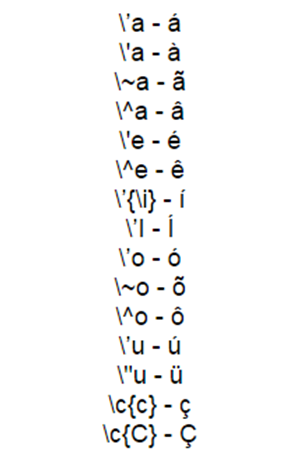
\includegraphics[scale=1.0]{USPSC-img/USPSC-AcentuacaoLaTeX.png} \\
	Fonte: \citeonline{comandos}
	\end{center}	
\end{figure}

\end{anexosenv}


%---------------------------------------------------------------------
% INDICE REMISSIVO
%--------------------------------------------------------------------
%% USPSC-IndicexRemissivosTutorial.tex
% ---
% Inicia os Índices Remissivos
% ---
%---------------------------------------------------------------------
% INDICE REMISSIVO
%--------------------------------------------------------------------
\phantompart
\printindex
%---------------------------------------------------------------------


%---------------------------------------------------------------------

\end{document}
